% modified from NeurIPS 2022 Latex template
% authors: Yixin Zhu (yixin.zhu@pku.edu.cn), Liangru Xiang
% v1.0: 2022.07.21

\documentclass{article}
\PassOptionsToPackage{numbers,compress}{natbib}
\usepackage[final]{template22}
\input{config.tex}

\title{Generate SPICE netlists based on the images of analog circuits}
\newcommand{\runningauthor}{Mengyao Zhang}
\newcommand{\runningid}{2025-0067}

\author{%
  Mengyao Zhang\\ % \thanks{Zichen Kong.} \\
  School of Physics\\
  Peking University\\
  \texttt{mengyao@stu.pku.edu.cn} \\
  % examples of more authors
  % \And
  % Coauthor \\
  % Affiliation \\
  % Address \\
  % \texttt{email} \\
  % \AND
  % Coauthor \\
  % Affiliation \\
  % Address \\
  % \texttt{email} \\
  % \And
  % Coauthor \\
  % Affiliation \\
  % Address \\
  % \texttt{email} \\
  % \And
  % Coauthor \\
  % Affiliation \\
  % Address \\
  % \texttt{email} \\
}

\begin{document}
\maketitle

The video report is located at \url{https://disk.pku.edu.cn/link/AABFFB828A7D204E6EB5785974A6A2C892}. 

\begin{abstract}
This report explores the automated generation of SPICE netlists from images of analog circuits, with a focus on improving existing algorithms for application to Razavi's textbook. 
While analog circuits form the backbone of many electronic devices, converting their diagrams into SPICE netlists—a textual representation essential for simulation and analysis—poses significant challenges due to variations in image quality, noise, and non-standardized conventions. 
Building on the work of Shi et al., this report introduces key enhancements, including optimized template matching, noise removal techniques, and refined handling of components like operational amplifiers. 
The improved algorithm achieves an average component detection rate of 70\% on printed images, rising to 84\% with higher-quality PDF versions. 
Despite these advancements, persistent limitations such as PMOS/NMOS confusion and challenges with non-standard circuits highlight the need for further research. 
The report also discusses the inadequacy of large pre-trained models for circuit interpretation and underscores the lack of standardization in academic literature. 
These findings contribute to ongoing efforts to automate circuit analysis and facilitate the development of datasets for training large language models in electronic design.
\end{abstract}

\section{Introduction}\label{sec:introduction}

Analog circuits are electrical circuits that process continuous signals, in contrast to digital circuits which operate with discrete values. 
These circuits form the foundation of numerous everyday electronic devices, including radios, amplifiers, and sensors. 
By employing components such as resistors, capacitors, inductors, transistors, and operational amplifiers, analog circuits manipulate voltage and current in a smooth, continuous manner.

SPICE (Simulation Program with Integrated Circuit Emphasis) serves as a widely adopted tool for simulating and analyzing electronic circuits. 
A SPICE netlist provides a textual representation of an electronic circuit, detailing its components, their interconnections, and the necessary simulation parameters. 
An example of such a netlist is illustrated in \cref{fig:spice_example}.

\begin{figure}[htbp]
    \centering
    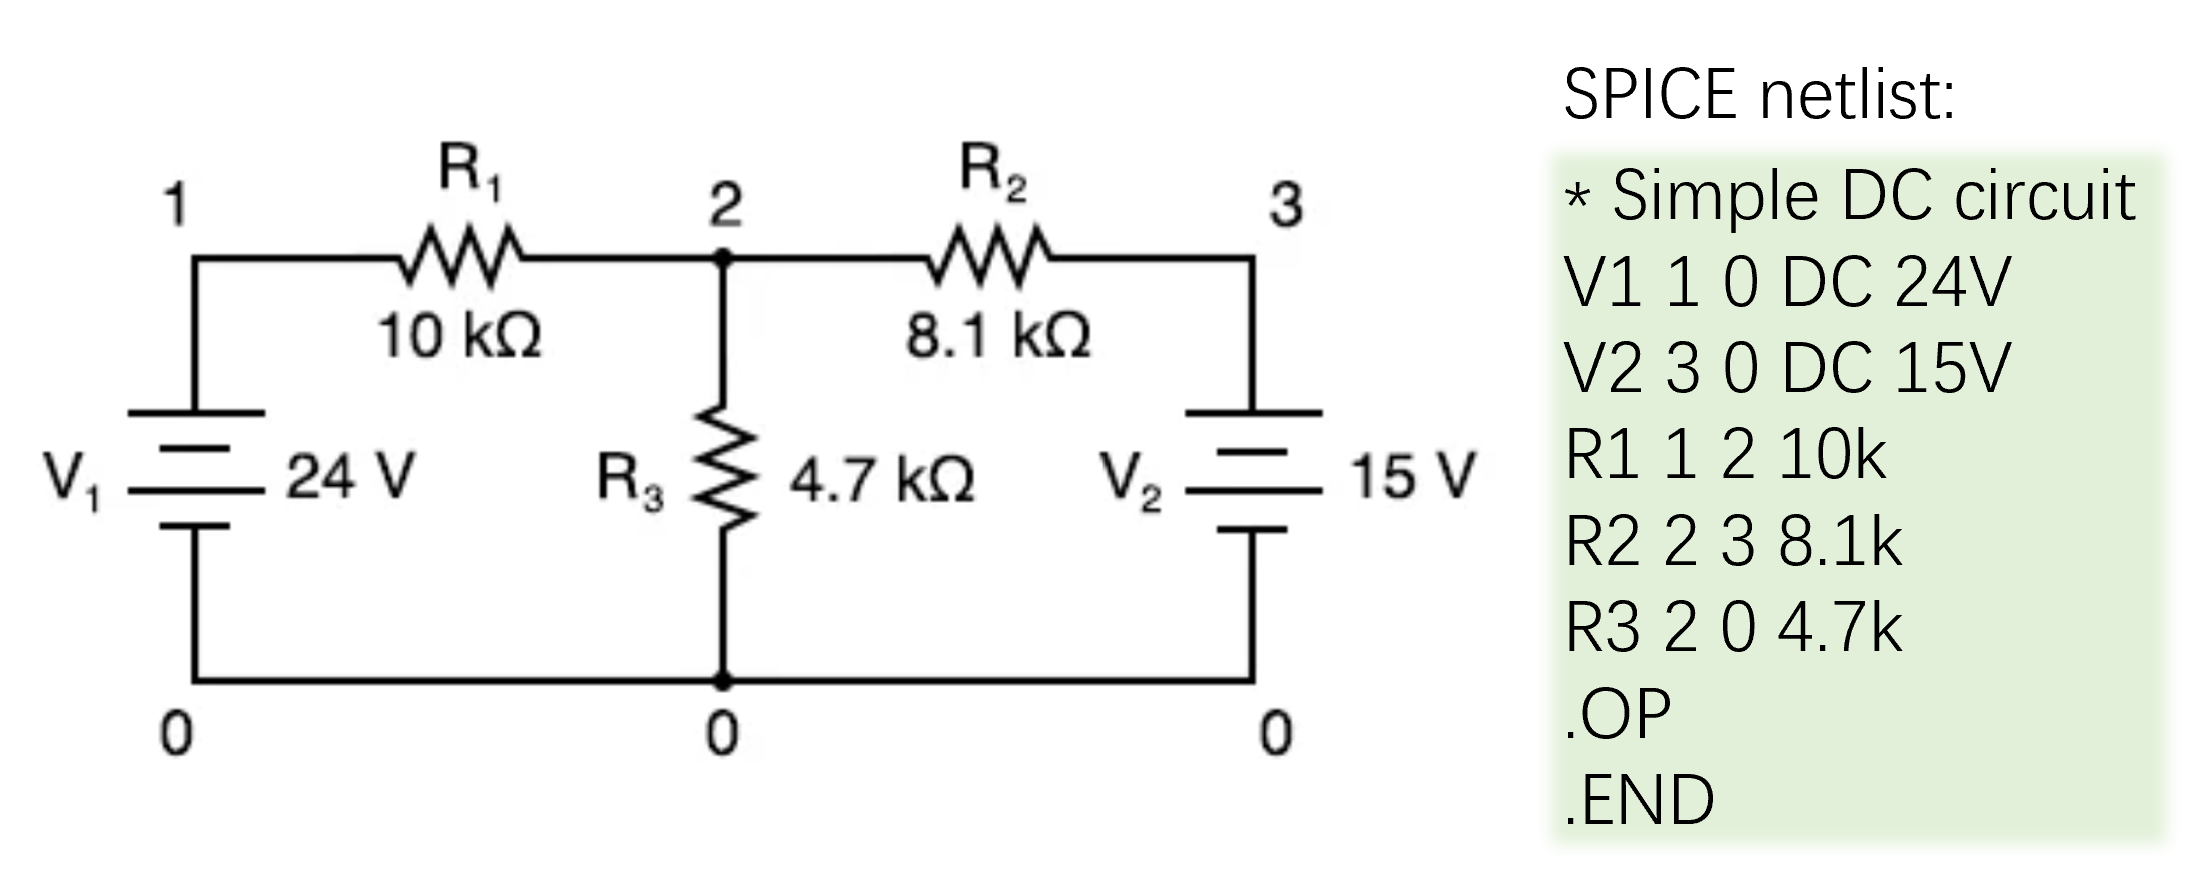
\includegraphics[width=0.5\textwidth]{figures/spice_example.png}
    \caption{\textbf{An example of a SPICE netlist.}\\
    Left is a topological circuit diagram, the right is the corresponding SPICE netlist.
    Each line of the netlist represents a component, with its type, name, and connections to other components.
    For some components not symmetric in pins, certain order of pins in the netlist is required, as is the case for NMOS and PMOS transistors etc.
    The circuit diagram is adapted from \cite{example_circuits}.}
    \label{fig:spice_example} 
\end{figure}

The conversion of circuit diagrams into SPICE netlists requires several key steps: identifying components, determining their connections, and formatting this information into the netlist structure. 
This conversion process is crucial for efficient electronic design and analysis. 
Furthermore, it represents an essential step in constructing datasets for training large language models (LLMs) to comprehend and generate SPICE netlists.

This work focuses specifically on the automated conversion of circuit diagrams-particularly those from textbooks or literature pages—into SPICE netlists. 
However, the process encounters challenges when handling images from research papers, which exhibit significant variation and lack standardized conventions. 
Consequently, the primary objective of this work is to apply an improved algorithm to Razavi's book \cite{razavi2003}, a task not addressed in previous efforts.

The remainder of this report is organized as follows. 
\cref{sec:review_of_current_work} reviews existing approaches for generating SPICE netlists from circuit images, forming the foundation for subsequent work. 
\cref{sec:improvements} examines the limitations of the algorithm presented in \cref{sec:review_of_current_work} and describes the corresponding enhancements implemented for Razavi's book. 
To achieve higher accuracy and stability, we utilize a PDF version of the textbook featuring higher-quality images in the conversion process. 
We evaluate results from both printed and PDF versions using a "component detection rate" metric. 
\cref{sec:challenges} analyzes persisting limitations of the improved algorithm and outlines future work, while also discussing the difficulties large models face in processing circuit images. 
Finally, \cref{sec:conclusion} concludes the report.

\section{Review of current work}\label{sec:review_of_current_work}

Shi \etal \cite{shi2024amsnet} recently proposed a method for generating SPICE netlists from analog circuit images in textbooks and literature. 
Their approach combines template-matching, breadth-first search (BFS), and several detailed processing steps. 
This section provides a brief overview of their pipeline. 

\cref{subfig1:shi_work_pipeline} illustrates the general workflow, which comprises four main stages:

(1) image extraction, filtering and preprocessing, 

(2) component and boundary detection, 

(3) building groups of connected components and corresponding pins,

(4) postprocessing to fix the net intersections and to merge the same points. 

These steps are demonstrated in \cref{subfig2:shi_grouping,subfig3:shi_pin_ordering,subfig4:shi_intersection} and are elaborated below.

\subsection{Preprocessing}

The process begins with collecting analog circuit images from textbooks or papers, 
which are converted to binary images (pixel values 0 for black or 1 for white). 
Individual components are then manually cropped from these images. 
Most cropped components undergo automatic rotation at $90^\circ$, $180^\circ$, and $270^\circ$ to minimize manual labeling effort.

These cropped elements serve as templates, named following conventions such as "nmos\_90\_1", where:
\begin{itemize}
\item "nmos" indicates the component type
\item "90" specifies the rotation angle
\item"1" represents the template index (starting from 0)
\end{itemize}
Multiple templates with varying rotation angles enable direction identification during subsequent template matching, 
while multiple indices accommodate slight shape variations for improved matching accuracy.

\subsection{Component and boundary detection}

Component detection employs OpenCV's $cv2.matchTemplate$ function for template matching. 
Textbook images, benefiting from uniform printing and consistent formatting, require only a few templates to cover all components. 
Notably, all node types-including T-junctions and cross-junctions-are treated as components and detected similarly. 
Examples appear in \cref{subfig1:shi_net-black_1110} and \cref{subfig2:shi_net-black_1111}.

Stricter tolerance values are applied for "VDD" components (illustrated in \cref{subfig3:shi_vdd_0}), which are particularly susceptible to misidentification. 
When boundaries overlap, the system retains the match with the highest $cv2.matchTemplate$ score while discarding others.

\begin{figure}[htbp]
    \centering
    \begin{subfigure}[b]{0.2\textwidth}
        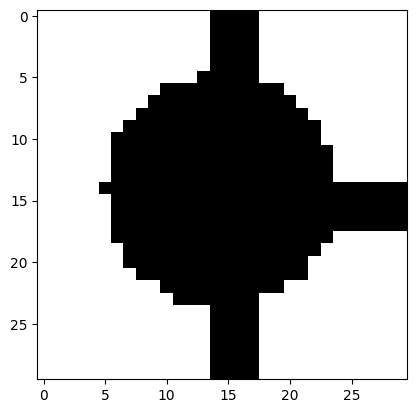
\includegraphics[width=\linewidth]{figures/shi_net-black_1110.png}
        \caption{}
        \label{subfig1:shi_net-black_1110}
    \end{subfigure}
    \begin{subfigure}[b]{0.2\textwidth}
        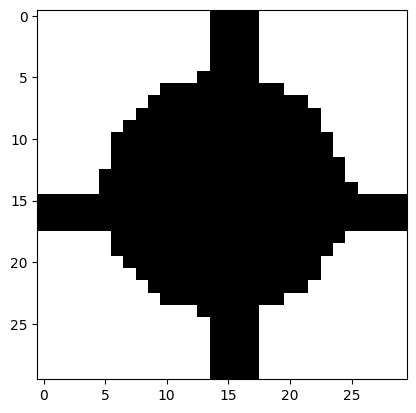
\includegraphics[width=\linewidth]{figures/shi_net-black_1111.png}
        \caption{}
        \label{subfig2:shi_net-black_1111}
    \end{subfigure}
    \begin{subfigure}[b]{0.2\textwidth}
        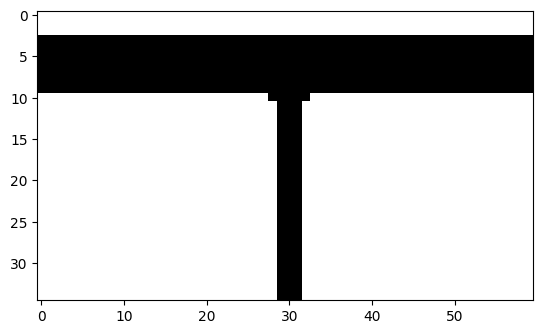
\includegraphics[width=\linewidth]{figures/shi_vdd_0.png}
        \caption{}
        \label{subfig3:shi_vdd_0}
    \end{subfigure}
    \caption{\textbf{Some of the templates used in Shi's work.}\\
    (a) and (b) are T-junctions and cross-junctions, which are treated as components.
    (c) is the template for "VDD", which is more prone to be misidentified, and thus stricter tolerance values are used.}
    \label{shi_}
\end{figure}

\begin{figure}[htbp]
    \centering
    \begin{subfigure}[b]{0.9\textwidth}
        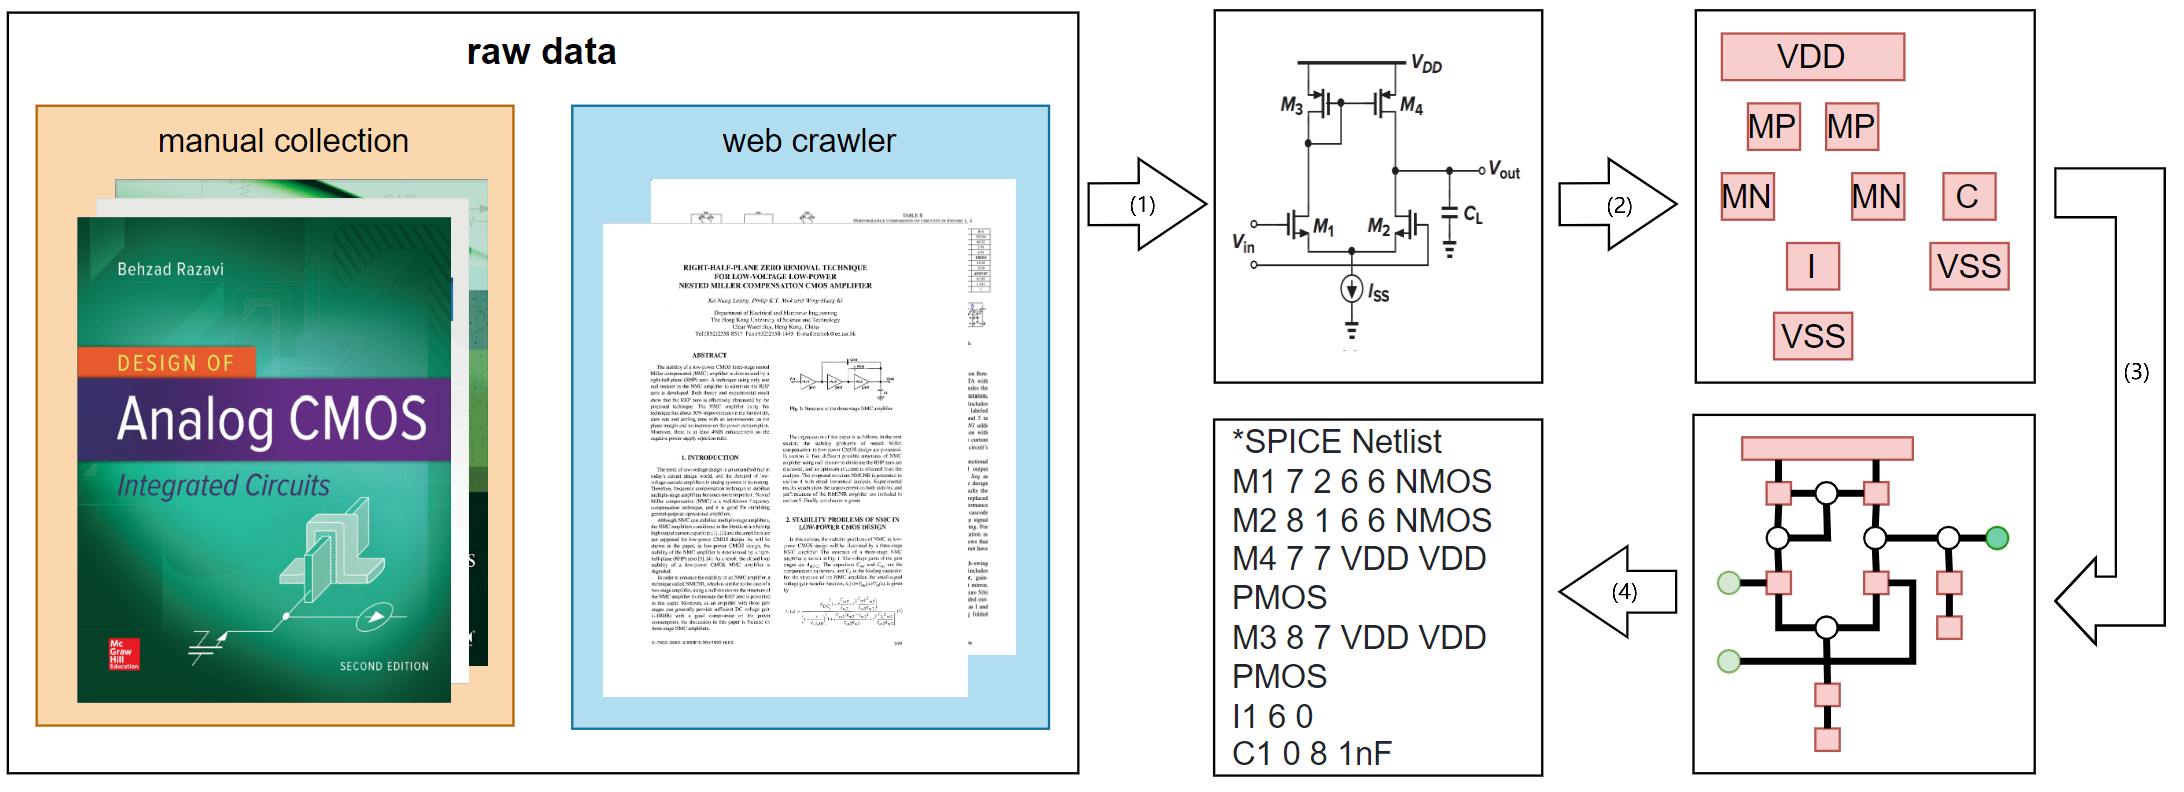
\includegraphics[width=\linewidth]{figures/shi_work_pipeline.png}
        \caption{}
        \label{subfig1:shi_work_pipeline}
    \end{subfigure}
    \begin{subfigure}[b]{0.3\textwidth}
        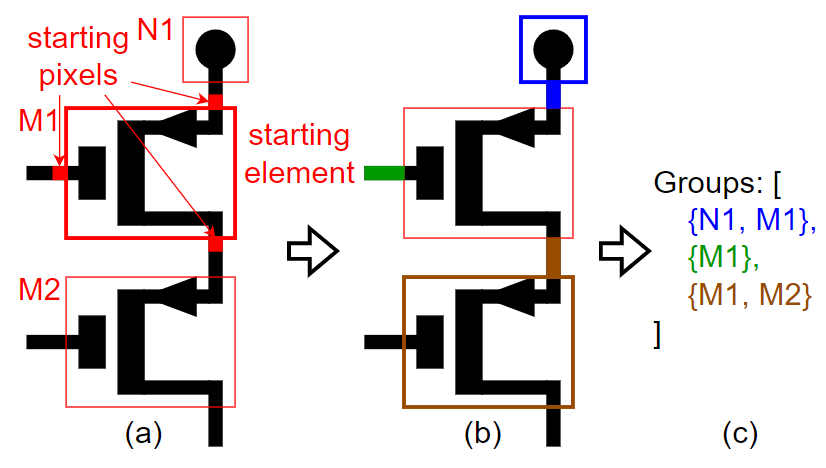
\includegraphics[width=\linewidth]{figures/shi_grouping.png}
        \caption{}
        \label{subfig2:shi_grouping}
    \end{subfigure}
    \begin{subfigure}[b]{0.25\textwidth}
        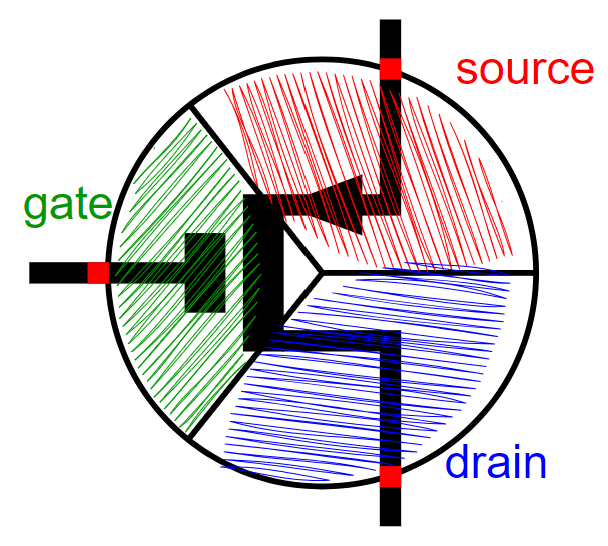
\includegraphics[width=\linewidth]{figures/shi_pin_ordering.png}
        \caption{}
        \label{subfig3:shi_pin_ordering}
    \end{subfigure}
    \begin{subfigure}[b]{0.35\textwidth}
        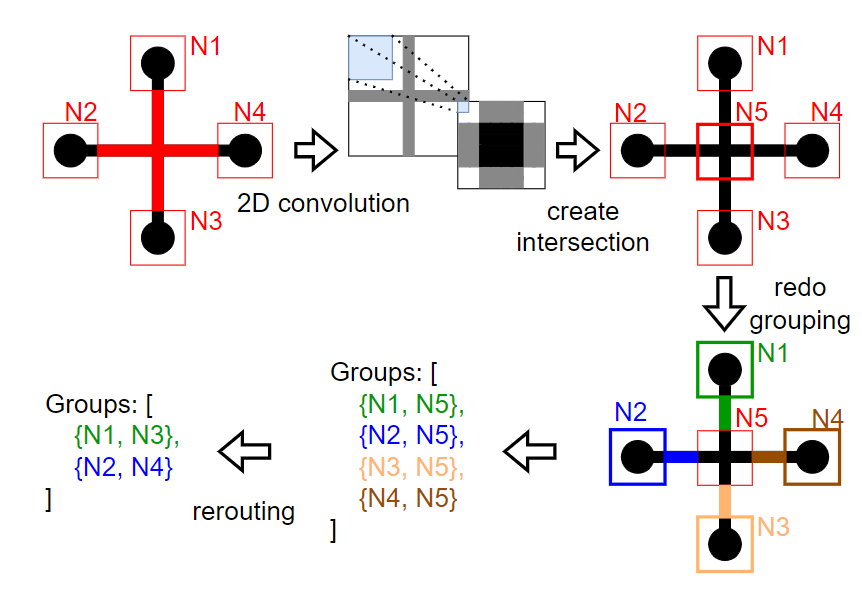
\includegraphics[width=\linewidth]{figures/shi_intersection.png}
        \caption{}
        \label{subfig4:shi_intersection}
    \end{subfigure}
    \caption{\textbf{Review of Shi's work.}\\
    \textbf{(a) Pipeline of Shi's work to generate netlists.}
        A number of circuits images are extracted from textbooks or papers. 
        Then the flow detects the components and nets from the images, and generates full netlists.
        (1) image extraction and filtering, (2) component detection, (3) net identification, (4) netlist generation. \\
    \textbf{(b) Grouping components for net detection.}
        Search from the intersection of a component boundary and a wire, until running into another component boundary, 
        thereby grouping all connected components.\\
    \textbf{(c) Pin ordering.}
        Find the angle of the intersection of boundaries and wires relative to the center of the components. The pins are then ordered and stored with the connection groups. \\
    \textbf{(d) Resolving intersection cases.}
        If more than two pins are connected into one group, and assuming the detection process hasn't omitted any "T" junctions or cross junctions etc, 
        the intersection is to be resolved by imposing a 2d convolution searching involved wirings. 
        Next, the opposite sides of an intersection are connected and the original group becomes two groups. 
        This process is repeated until all intersections are resolved and each group contains only two components.\\
        The figures are adapted from \cite{shi2024amsnet}.}
    \label{fig:shi_work}
\end{figure}

\subsection{Building groups of connected components and corresponding pins}

The algorithm initiates a BFS from wire-boundary intersections to identify components connected via wiring, thereby constructing connected component groups. 
Component bounding boxes include directional information, enabling the algorithm to determine connection pins based on angular ranges between boundary box-wire intersections and device center points.

These connected components and their corresponding pins are stored in a dictionary structure.

\subsection{Postprocessing}

Assuming no undetected T-junctions or cross-junctions, cases with more than two connected pins typically represent wire intersections rather than true junctions. 
The algorithm locates these intersections by performing 2D convolution along the responsible wiring segments, identifying denser regions. 
The original groups are then split by connecting opposite sides of each intersection, repeating this process until all intersections are resolved and each group contains exactly two components.

Finally, the system merges groups sharing equivalent points and generates the netlist from the resulting connection groups.

\section{Improvements of current work and application to Razavi's book}\label{sec:improvements}

The algorithm proposed by Shi \cite{shi2024amsnet} was tested on various images from both textbooks and research papers. 
Results revealed that circuit figures from papers lack uniform organization and standardized conventions, presenting numerous conversion challenges as detailed in \cref{sec:challenges}.

Consequently, this work focuses on applying an improved version of the algorithm to Razavi's book \cite{razavi2003}, addressing gaps in previous implementations.

\subsection{Identified limitations and implemented enhancements}

\subsubsection{Template matching optimization}

The original algorithm employs OpenCV's $cv2.matchTemplate$ function, which scans images using a template-sized window for component detection. 
A significant limitation emerged when template dimensions mismatched actual component sizes in the images.

To address this, we implemented template resizing, scaling templates between 1.0$\times$ to 1.05$\times$ their original dimensions. 
While this adjustment shows modest impact on well-formatted textbook images, it proves essential for potential applications to research paper figures.

\subsubsection{Noises (text, dashed lines and other unwanted information) removal}\label{subsubsec:noises}

Circuit figures in Razavi's book, like those in research papers, contain extraneous elements such as text labels, dashed lines, and other annotations that don't contribute to the topological structure. 
These elements, termed "noises" in this work, can significantly impact conversion accuracy. 
Example noise patterns are shown in \cref{subfig1:noise_example1,subfig2:noise_example2,subfig_addition:noise_example3}.

While Shi's approach minimizes noise interference through careful template cropping, this proves insufficient for Razavi's book, as further discussed in \cref{subsec:tight_boundaries_insufficient}.

Our enhanced preprocessing stage systematically removes textual and graphical annotations while preserving circuit components. 
The algorithm:
\begin{itemize}
\item Uses a 44-pixel line convolution kernel to detect wiring segments
\item traverses the circuits via BFS starting from all the detected wiring segments
\item Retains critical symbols (current sources, ground connections, which may have isolated parts that are not traversed in BFS) via targeted template matching
\item Maintains polarity markers (+, -) through optimized kernel convolution
\end{itemize}
The preprocessing results are visualized in \cref{fig:remove_noises}, 
with red lines highlighting detected wiring segments and their center points serving as BFS starting locations.

\begin{figure}[htbp]
    \centering
    \begin{subfigure}[b]{0.25\textwidth}
        \centering
        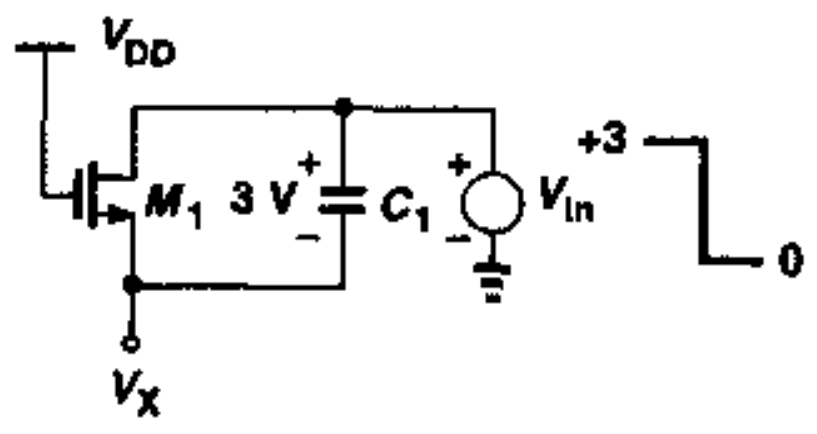
\includegraphics[width=\linewidth]{figures/noise_example1.png}
        \caption{}
        \label{subfig1:noise_example1}
    \end{subfigure}
    \begin{subfigure}[b]{0.35\textwidth}
        \centering
        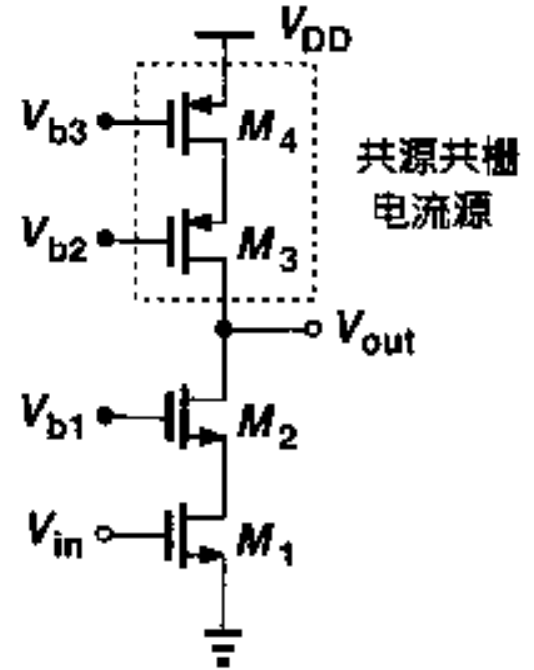
\includegraphics[width=0.5\linewidth]{figures/noise_example2.png}
        \caption{}
        \label{subfig2:noise_example2}
    \end{subfigure}
    \begin{subfigure}[b]{0.32\textwidth}
        \centering
        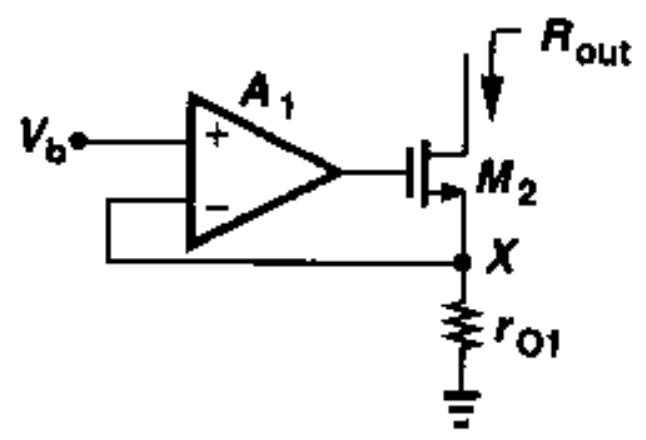
\includegraphics[width=\linewidth]{figures/noise_example3.png}
        \caption{}
        \label{subfig_addition:noise_example3}
    \end{subfigure}
    
    \caption{\textbf{Examples of noises in Razavi's book.}\\
        Such noises include texts, 
        dashed lines and other annotations, which are not part of the circuit topological structure, 
        but can affect the converting process. 
        The bound of OPAMP will inevitably include texts, indicated in (c).\\}
    \label{fig:noise}
\end{figure}

\begin{figure}[htbp]
    \centering
    \begin{subfigure}[b]{0.15\textwidth}
        \centering
        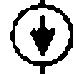
\includegraphics[width=\linewidth]{figures/current-arrow_0_0.jpg}
        \caption{}
        \label{subfig1:current-arrow_0_0}
    \end{subfigure}
    \begin{subfigure}[b]{0.15\textwidth}
        \centering
        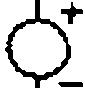
\includegraphics[width=\linewidth]{figures/voltage_0_0.jpg}
        \caption{}
        \label{subfig2:voltage_0_0}
    \end{subfigure}
    \begin{subfigure}[b]{0.15\textwidth}
        \centering
        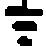
\includegraphics[width=\linewidth]{figures/gnd_0_0.jpg}
        \caption{}
        \label{subfig3:gnd_0_0}
    \end{subfigure}
    \begin{subfigure}[b]{0.15\textwidth}
        \centering
        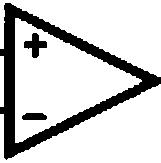
\includegraphics[width=\linewidth]{figures/opamp-3_0_0.jpg}
        \caption{}
        \label{subfig4:opamp-3_0_0}
    \end{subfigure}
    \caption{\textbf{Components to be specifically considered.}\\
    Before BFS and erasing, current sources, voltage sources, ground symbols and OPAMPs have isolated parts which should be preserved.\\
    \textbf{(a)} is the current source.\\
    \textbf{(b)} is the voltage source. \\
    \textbf{(c)} is the ground symbol.\\
    \textbf{(d)} is the OPAMP with three pins.}
    \label{fig:isolated_of_components}
\end{figure}

\begin{figure}[htbp]
    \centering
    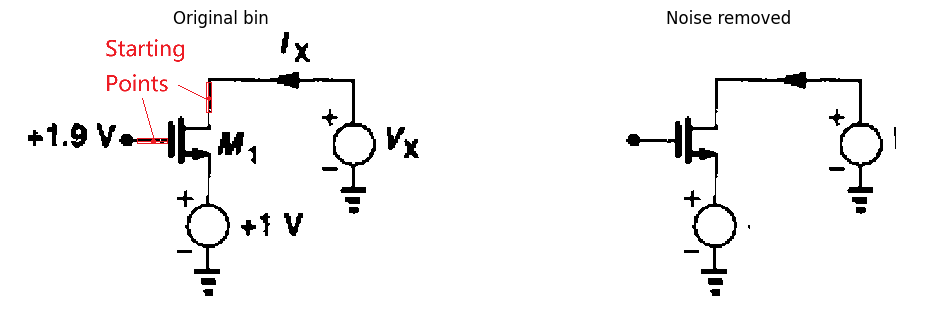
\includegraphics[width=0.7\linewidth]{figures/remove_noises.png}
    \caption{\textbf{Visualisation of noise-removing process.}\\
    The red lines in rectangular boxes are some of the wirings detected by convolution,
    their centers being the starting points.
    Only two of such lines and starting points are shown in the figures. 
    Components consisting of isolated parts are preserved, such as voltage sources and gnd symbols. 
    Starting points appear in both sides of NMOS, which contains two isolated parts, therefore eliminating the need to detect NMOS.}
    \label{fig:remove_noises}
\end{figure}

\subsubsection{Refined template matching parameters}

Beyond template resizing, we implemented component-specific threshold adjustments for matching accuracy. 
While the original code only customized thresholds for VDD components, our improvements include:

\begin{itemize}
\item Optimized template cropping dimensions. 
Take black nodes as an example, of which a tight cropping may lead to misidentification, as mentioned in \cref{subsec:tight_boundaries_insufficient}.
However, too large a boundary may lead to boundary overlapping between two closely placed components, some components not detected as a result.
\item Balanced threshold sensitivity to minimize both false positives and missed detections. 
In the final algorithm, thresholds for VDD, current arrows, nodes and junctions are set to 0.9, 0.9, 0.82, 0.82 respectively 
while those for other components are set to 0.75.
\item Expanded template libraries to accommodate varying component representations
\end{itemize}

Complex relationships exist between thresholds, cropping dimensions and the number of templates. 
So extensive testings were conducted to find the balance between these parameters.

\subsubsection{Operational amplifier handling}

The original implementation didn't address OPAMP components, examples of which appear in \cref{subfig1:opamp-2_0_0,subfig2:opamp-3_0_0}. 
After evaluating multiple approaches, we retained template matching as the most effective solution, with these enhancements:

\begin{itemize}
\item Explicit pin ordering (shown in \cref{subfig3:opamp_pins}) to handle asymmetric configurations
\item Multi-scale template matching to accommodate size variations
\item Setting a lower threshold for OPAMP alone
\item Priority-based conflict resolution (OPAMPs over VDD in boundary merging, since OPAMPs are prone to be locally identified as VDDs)
\end{itemize}

\begin{figure}[htbp]
    \centering
    \begin{subfigure}[b]{0.18\textwidth}
        \centering
        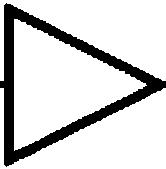
\includegraphics[width=\linewidth]{figures/opamp-2_0_0.jpg}
        \caption{}
        \label{subfig1:opamp-2_0_0}
    \end{subfigure}
    \begin{subfigure}[b]{0.18\textwidth}
        \centering
        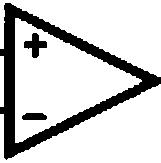
\includegraphics[width=\linewidth]{figures/opamp-3_0_0.jpg}
        \caption{}
        \label{subfig2:opamp-3_0_0}
    \end{subfigure}
    \begin{subfigure}[b]{0.3\textwidth}
        \centering
        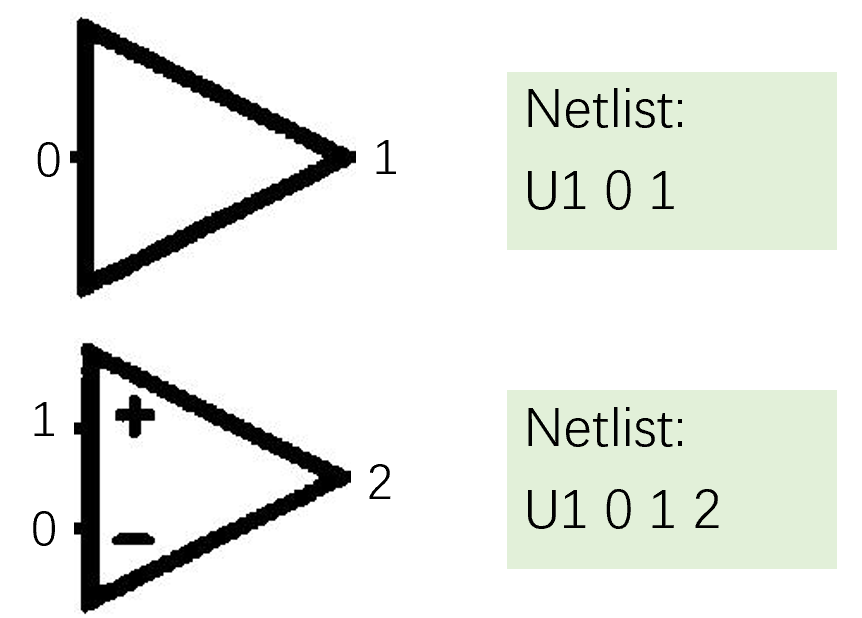
\includegraphics[width=\linewidth]{figures/opamp_pins.png}
        \caption{}
        \label{subfig3:opamp_pins}
    \end{subfigure}
    \caption{\textbf{Examples of OPAMPs in Razavi's book.}\\
    \textbf{(a)} is an OPAMP with two pins, which is not symmetric in pins.\\
    \textbf{(b)} is an OPAMP with three pins, which is also not symmetric in pins.\\
    \textbf{(c)} shows the rule of pins-ordering for OPAMPs. Here OPAMPs are noted as 'U'.}
    \label{fig:opamp_example}
\end{figure}

\subsection{Performance evaluation on Razavi's book}\label{sec:performance_evaluation}

The refined algorithm, incorporating all aforementioned improvements, was applied to Razavi's book circuits. 
Sample results appear in \cref{fig:netlist_result}, with unsuccessful cases analyzed in \cref{sec:challenges}.

We quantified performance using the following metric:
\begin{definition}
Component Detection Rate: The ratio of correctly identified components to total components in the circuit, where components include all templated elements (resistors, junctions, OPAMPs, etc.).
\end{definition}

This comprehensive metric inherently accounts for connection accuracy (since junctions are also treated as components), making additional connectivity measures unnecessary. 
Evaluation on 10 randomly selected circuits yielded an average detection rate of 70\%. 
It's worth noticing that some unimportant components undetected doesn't affect the netlist generation (such as the nodes discussed below),
so 70\% is considered a satisfactory result. As more templates are cropped and labeled, this rate can be further improved. 
And if merely considering circuits not so complicated, the rate is even higher.
Primary factors affecting performance include:
\begin{itemize}
\item Undetected nodes and current arrows (due to conservative thresholding)
\item PMOS/NMOS confusion
\item Missed junctions (T-junctions, cross-junctions) due to high thresholds chosen in order to avoid false positives
\end{itemize}
Fotunately, while undetected nodes lower the component detection rate, 
they minimally impact netlist generation quality, as evidenced in \cref{fig:netlist_result}.

\begin{figure}[htbp]
    \centering
    \begin{subfigure}[b]{0.1\textwidth}
        \centering
        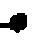
\includegraphics[width=\linewidth]{figures/net-black_1_0.jpg}
        \caption{}
    \end{subfigure}
    \begin{subfigure}[b]{0.1\textwidth}
        \centering
        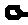
\includegraphics[width=\linewidth]{figures/net-white_100_0.jpg}
        \caption{}
    \end{subfigure}
    \begin{subfigure}[b]{0.16\textwidth}
        \centering
        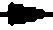
\includegraphics[width=\linewidth]{figures/current_270_0.jpg}
        \caption{}
    \end{subfigure}
    \caption{\textbf{Examples of nodes and current arrows in Razavi's book.}\\
    Undetected nodes and current arrows doesn't affect the netlist generation, because the end of a wire is always considered as a point equivalent to a node.}
    \label{fig:node_arrow_examples}
\end{figure}
\begin{figure}[htbp]
    \centering
    \begin{subfigure}[b]{0.96\textwidth}
        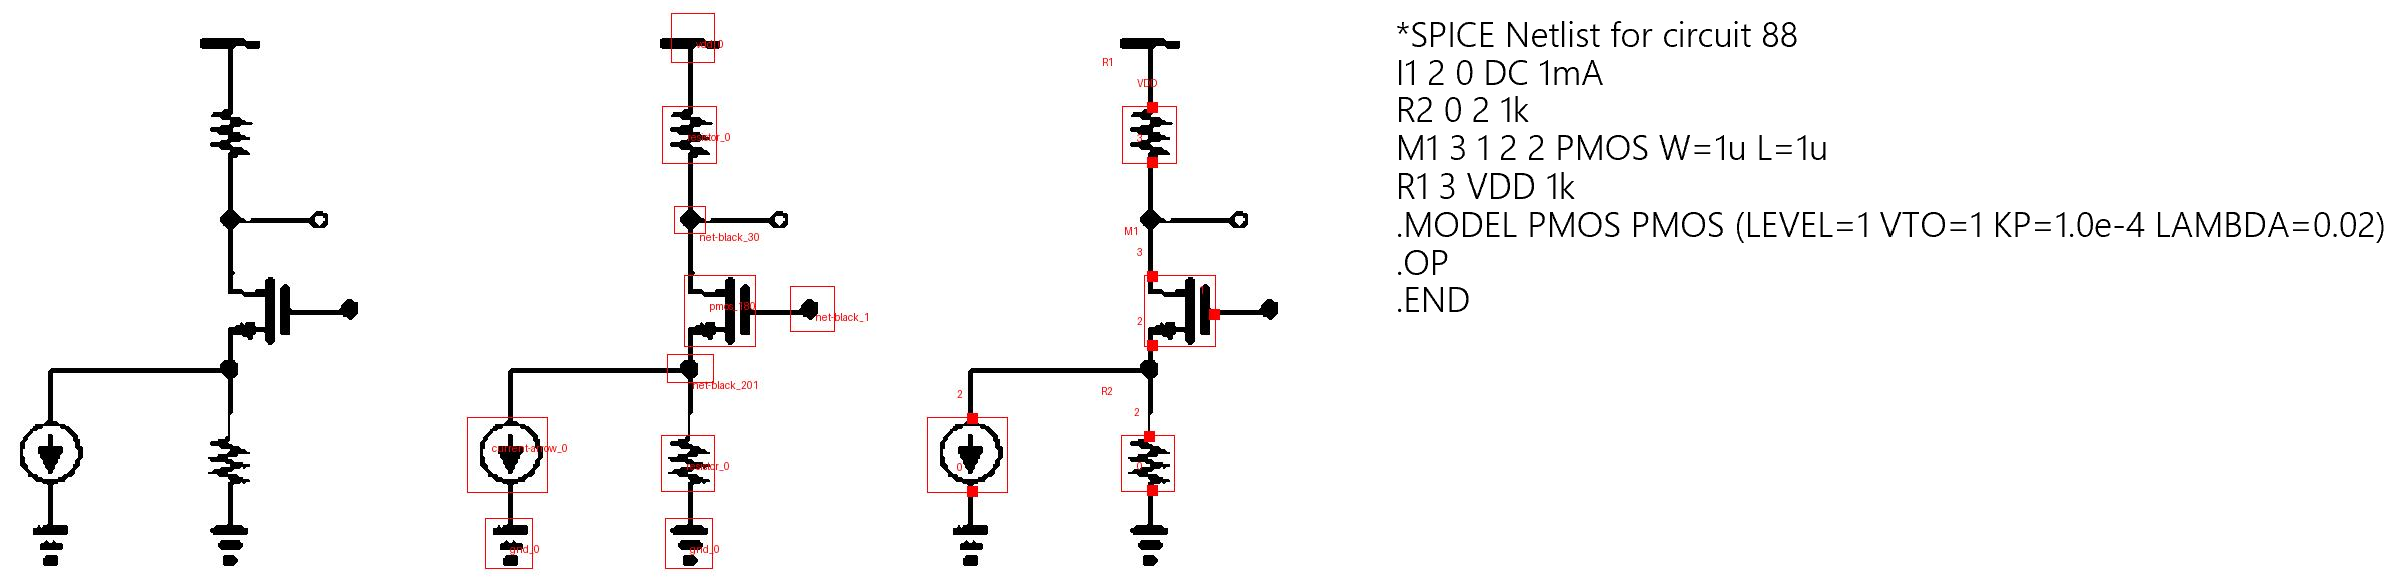
\includegraphics[width=\linewidth]{figures/netlist_result1.png}
        \caption{}
        \label{subfig1:netlist_result1}
    \end{subfigure}
    \begin{subfigure}[b]{0.96\textwidth}
        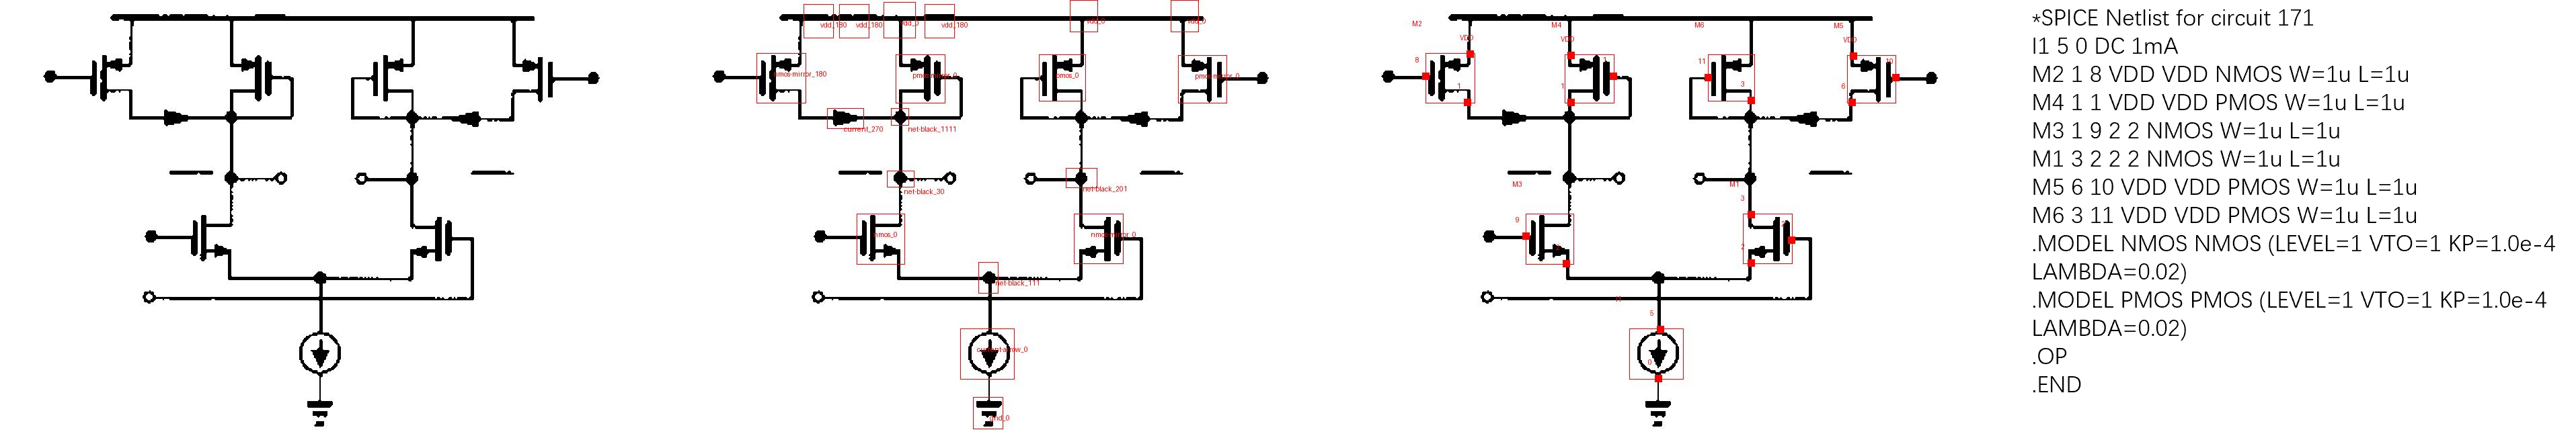
\includegraphics[width=\linewidth]{figures/netlist_result2.png}
        \caption{}
        \label{subfig2:netlist_result2}
    \end{subfigure}
    \caption{\textbf{Examples of generated SPICE netlists for complex circuits in Razavi's book.}\\
    The improved algorithm is applied on the images of Razavi's book, and work successfully on simple circuits.
    Results of two quite complex circuits are shown here.
    The netlists are generated almost successfully, with most of the components detected correctly.}
    \label{fig:netlist_result}
\end{figure}

\subsection{Images with better quality}

To enhance the algorithm's performance on critical components like PMOS, NMOS, and junctions, we sought higher quality image sources. 
After extensive searching, we obtained a PDF version of Razavi's book containing significantly clearer and smoother figures, as demonstrated in \cref{fig:printed_vs_pdf}. 
While some variations exist between the PDF and printed versions, we applied identical processing to both for comparative evaluation.

The improved image quality substantially enhances component detection accuracy. 
For instance, when reprocessing the circuit shown in \cref{subfig2:netlist_result2} using the PDF version, we observe measurable improvements illustrated in \cref{fig:netlist_comparison}. 
On average, this yields a 14 percentage point increase in component detection rate, from 70\% to 84\%.

\begin{figure}[htbp]
    \centering
    \begin{subfigure}[b]{0.4\textwidth}
        \centering
        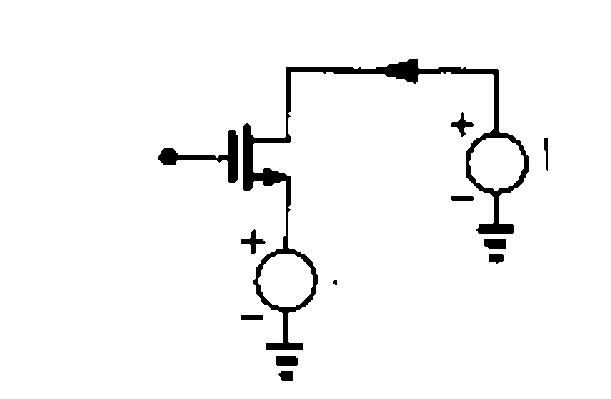
\includegraphics[width=\linewidth]{figures/printed_version.jpg}
        \caption{Printed version of Razavi's book.}
        \label{subfig1:printed_version}
    \end{subfigure}
    \begin{subfigure}[b]{0.4\textwidth}
        \centering
        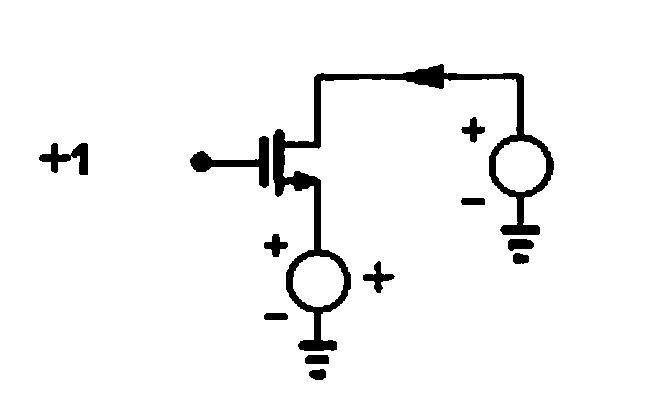
\includegraphics[width=\linewidth]{figures/pdf_version.jpg}
        \caption{PDF version of Razavi's book.}
        \label{subfig2:pdf_version}
    \end{subfigure}
    \caption{\textbf{Comparison between printed and PDF versions of Razavi's book.}\\
    The PDF version is clearer and smoother, which is more suitable for template matching.}
    \label{fig:printed_vs_pdf}
\end{figure}

\begin{figure}[htbp]
    \centering
    \begin{subfigure}[b]{0.96\textwidth}
        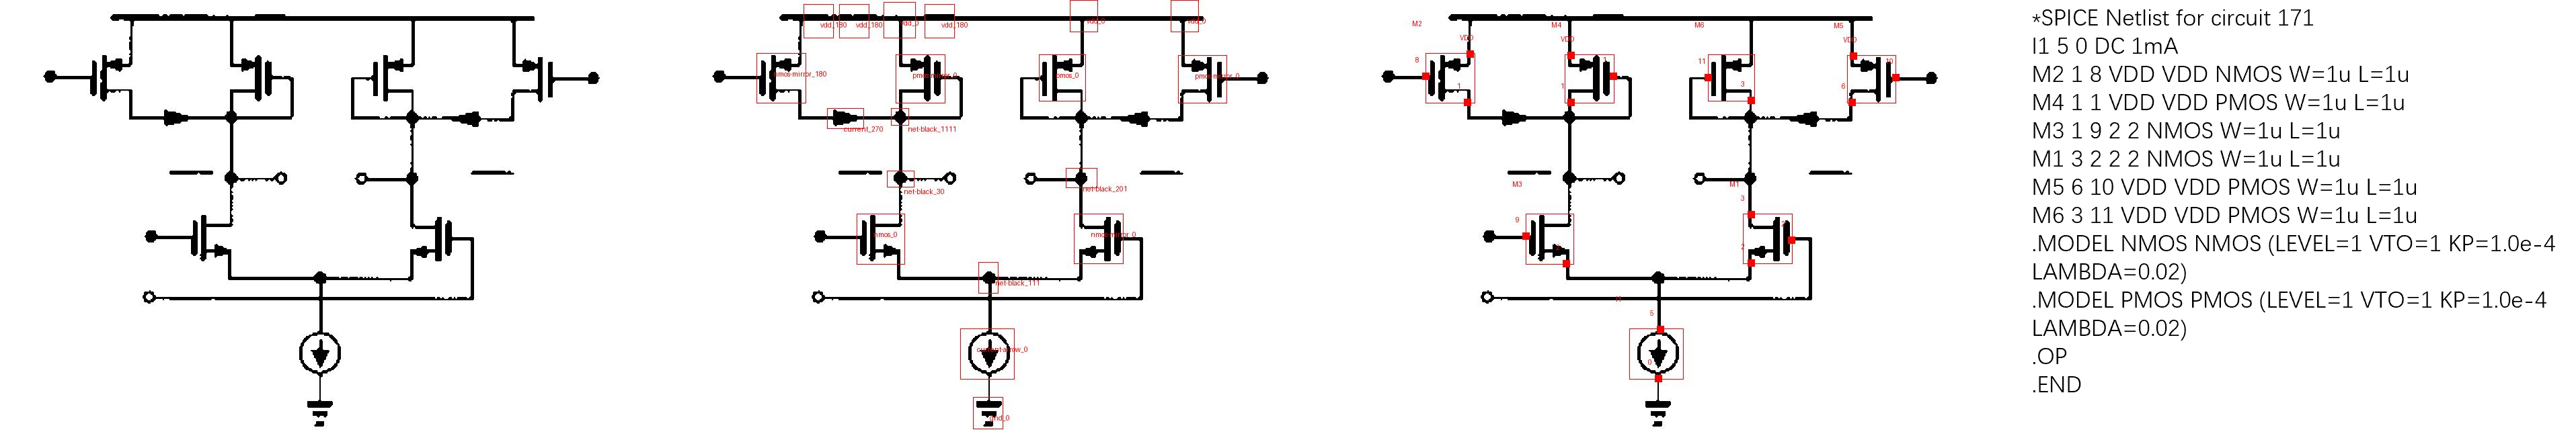
\includegraphics[width=\linewidth]{figures/netlist_result2.png}
        \caption{}
        \label{subfig1:netlist_comparison1}
    \end{subfigure}
    \begin{subfigure}[b]{0.96\textwidth}
        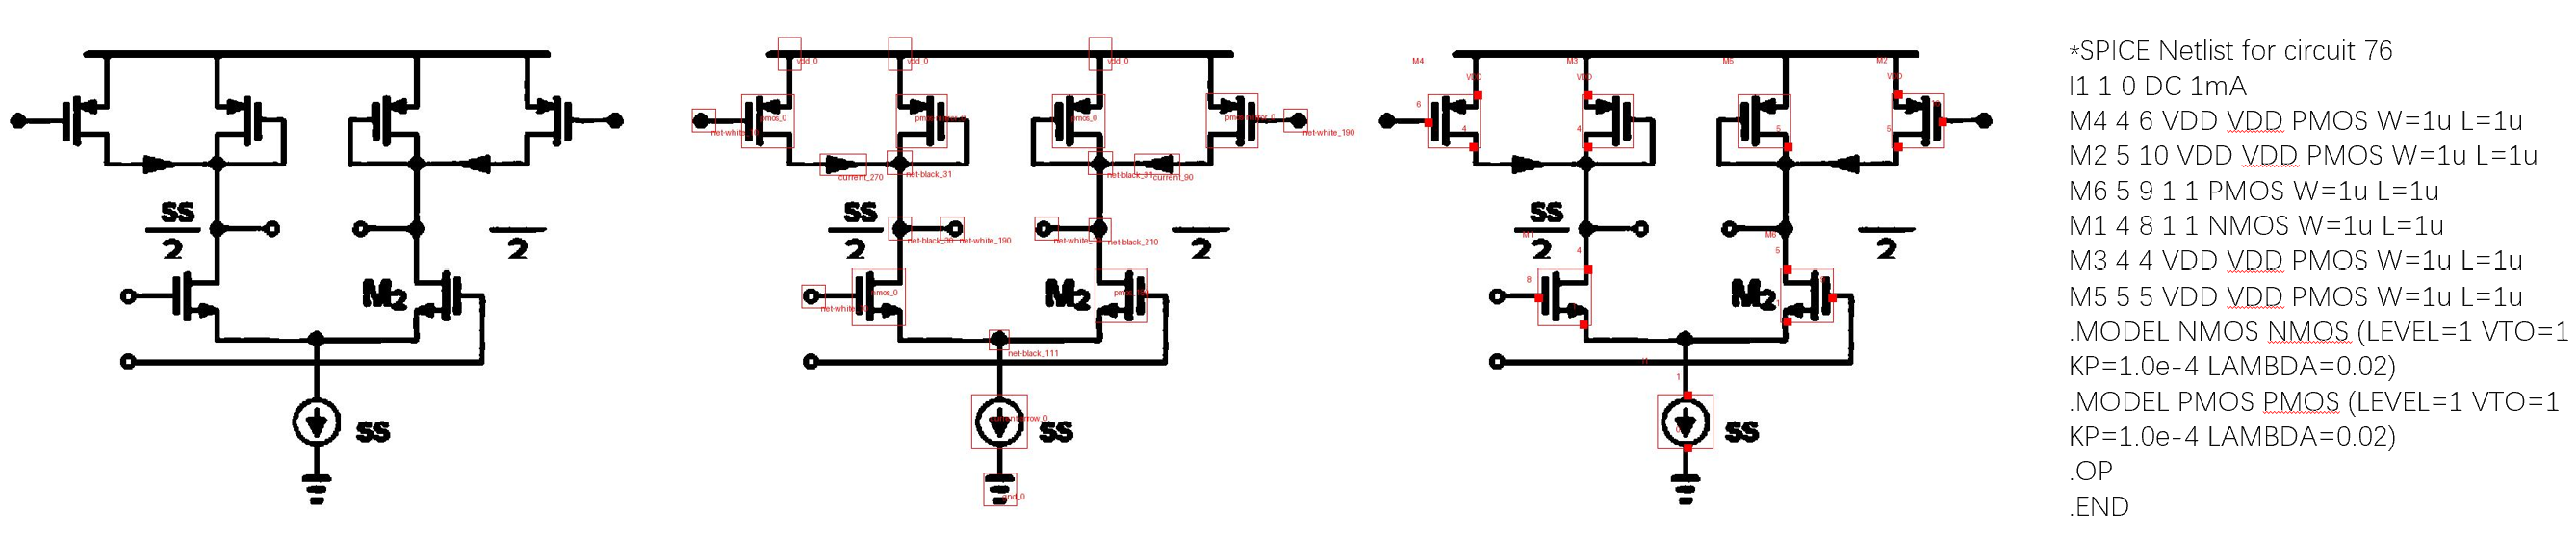
\includegraphics[width=\linewidth]{figures/netlist_result3.png}
        \caption{}
        \label{subfig2:netlist_comparison2}
    \end{subfigure}
    \caption{\textbf{Comparison of netlists generated from printed and PDF versions of Razavi's book.}\\
    \textbf{(a)} is the netlist generated from the printed version of Razavi's book, and 
    \textbf{(b)} is the netlist generated from the PDF version of Razavi's book.
    Apparently, the detection becomes more precise for PDF version.}
    \label{fig:netlist_comparison}
\end{figure}


\section{Challenges and future work}\label{sec:challenges}

Despite the algorithmic improvements detailed in \cref{sec:improvements}, several challenges persist. 
We also evaluated large pre-trained models on Razavi's circuit images, with unsatisfactory results discussed below.

\subsection{Limitations of the improved algorithm}

Even with superior quality PDF images, the algorithm exhibits persistent difficulties:
\begin{itemize}
\item Confusion between PMOS and NMOS due to their visual similarity
\item The rectangular boundary requirement in template matching forces merging of overlapping components, retaining only the highest-confidence detection 
(examples in \cref{subfig1:boundary_overlap1,subfig2:boundary_overlap2})
\end{itemize}

\begin{figure}[htbp]
    \centering
    \begin{subfigure}[b]{0.4\textwidth}
        \centering
        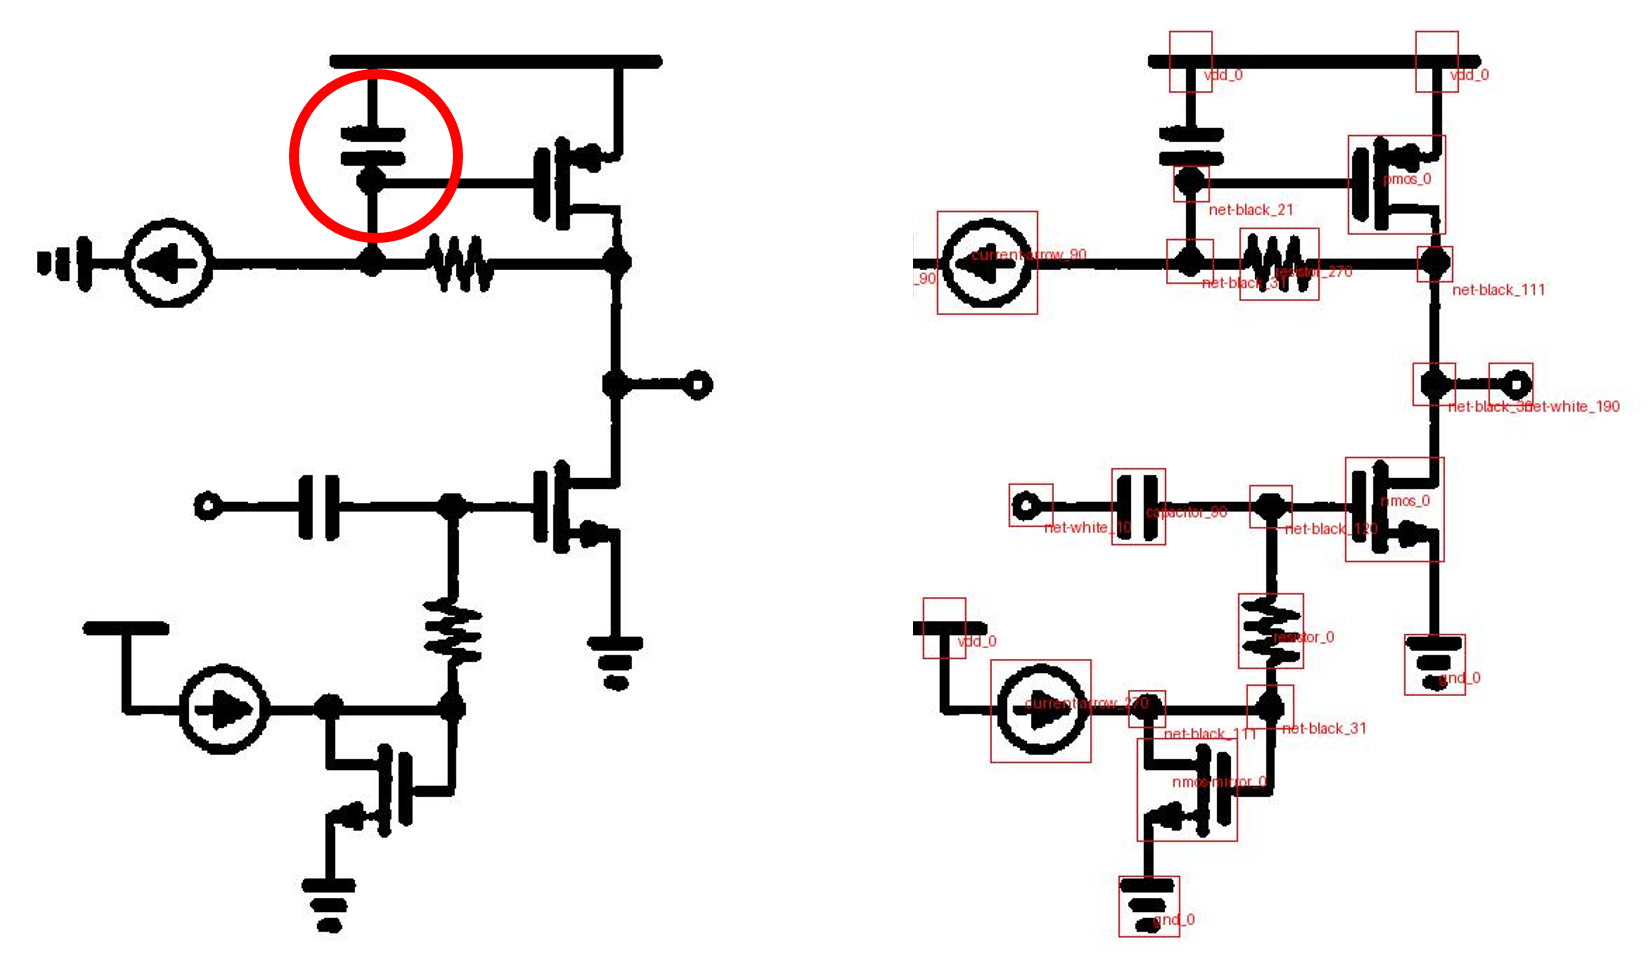
\includegraphics[width=\linewidth]{figures/boundary_overlap1.png}
        \caption{}
        \label{subfig1:boundary_overlap1}
    \end{subfigure}
    \begin{subfigure}[b]{0.22\textwidth}
        \centering
        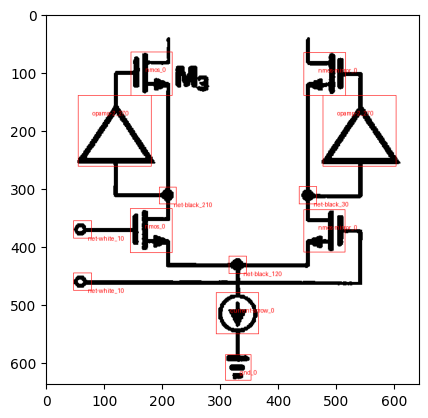
\includegraphics[width=\linewidth]{figures/boundary_overlap2.png}
        \caption{}
        \label{subfig2:boundary_overlap2}
    \end{subfigure}
    \begin{subfigure}[b]{0.4\textwidth}
        \centering
        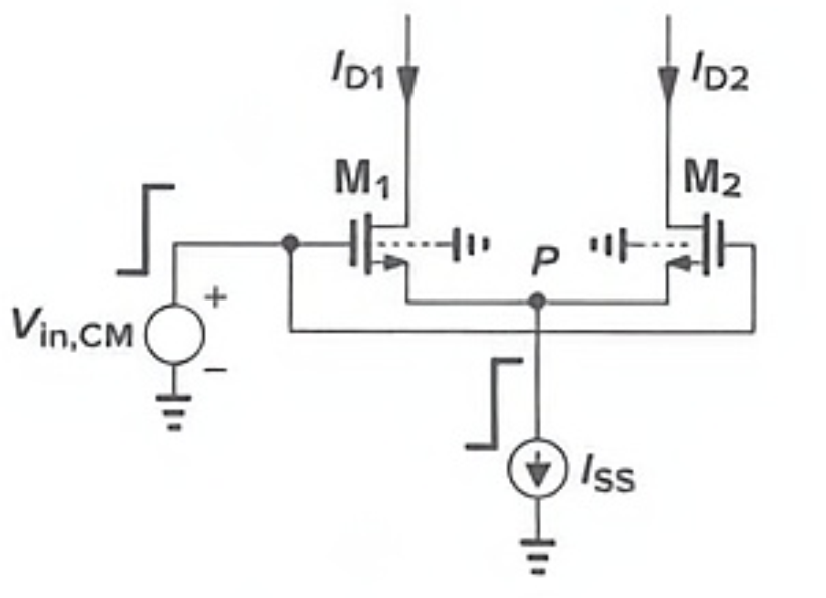
\includegraphics[width=\linewidth]{figures/extraordinary_dashed_line.png}
        \caption{}
        \label{subfig3:extraordinary_dashed_line}
    \end{subfigure}
    \begin{subfigure}[b]{0.4\textwidth}
        \centering
        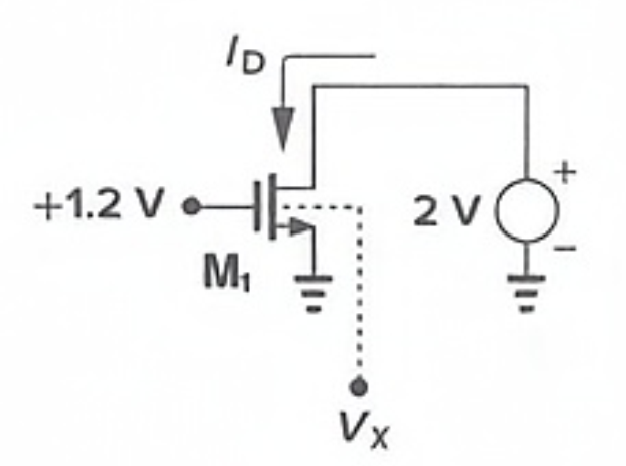
\includegraphics[width=\linewidth]{figures/extraordinary_dashed_line2.png}
        \caption{}
        \label{subfig4:extraordinary_dashed_line2}
    \end{subfigure}
    \begin{subfigure}[b]{0.4\textwidth}
        \centering
        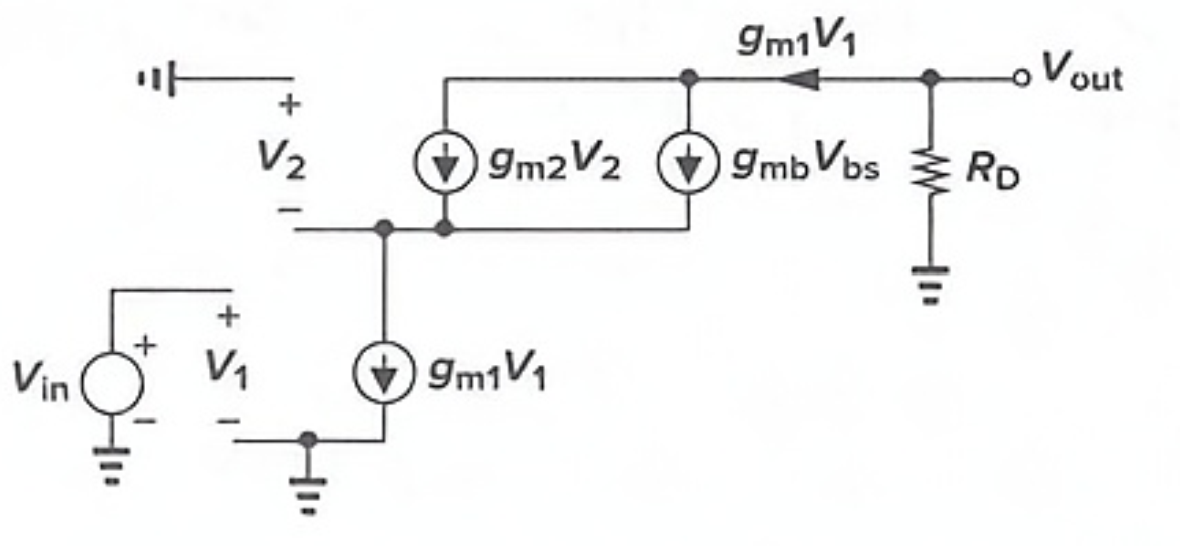
\includegraphics[width=\linewidth]{figures/extraordinary_controlled.png}
        \caption{}
        \label{subfig5:extraordinary_controlled}
    \end{subfigure}
    \begin{subfigure}[b]{0.22\textwidth}
        \centering
        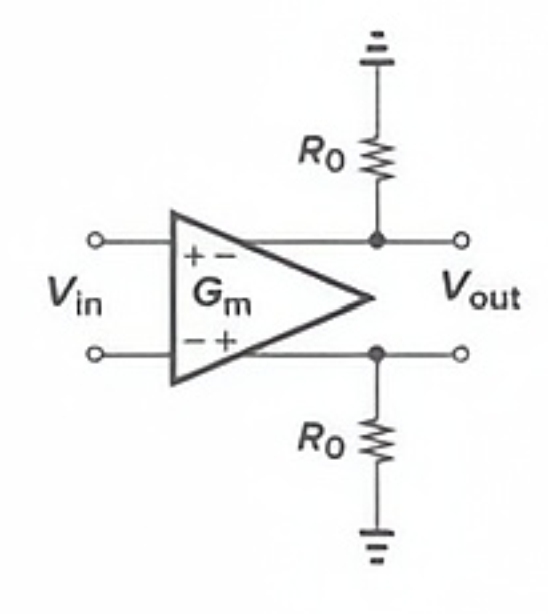
\includegraphics[width=\linewidth]{figures/extraordinary_controlled2.png}
        \caption{}
        \label{subfig6:extraordinary_controlled2}
    \end{subfigure}
    \begin{subfigure}[b]{0.4\textwidth}
        \centering
        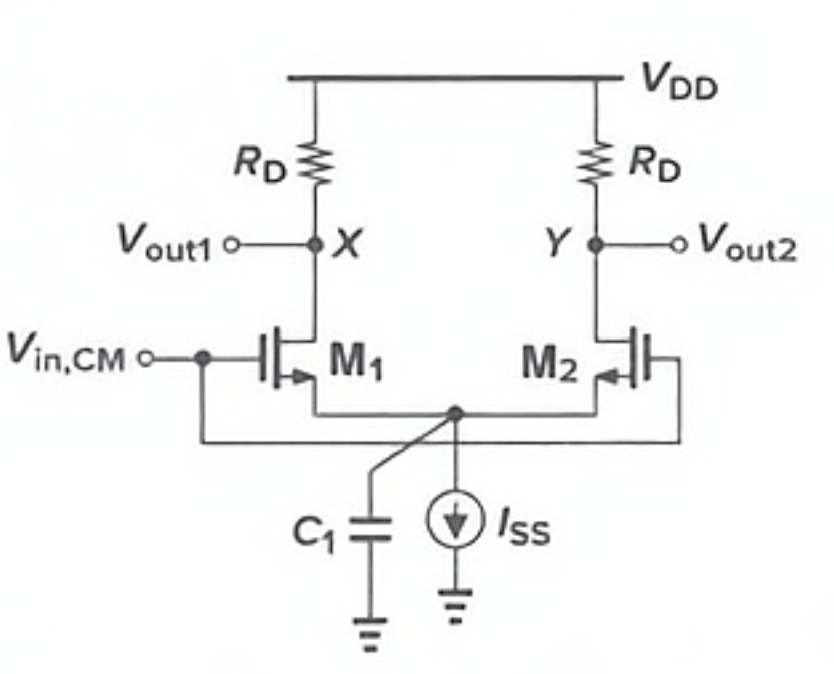
\includegraphics[width=\linewidth]{figures/extraordinary_junction.png}
        \caption{}
        \label{subfig7:extraordinary_junction}
    \end{subfigure}
    \caption{\textbf{Incapability of the algorithm.}\\
    \textbf{(a) Overlapping boundaries of a capacitor and a junction.}
    The boundaries overlap and only one of them is detected and boxed during the boundary merging process. \\
    \textbf{(b) Closely placed MOSFETs and OPAMPs.}
    The MOSFET and OPAMP are very close, a small deviation in the template matching may lead to merging the boundaries of them.
    Luckily, they are both detected here, narrowly.\\
    \textbf{(c) and (d) Dashed lines that aren't noises.}
    The dashed lines here carry information of pins of MOSFETs, which are not noises and shouldn't be erased.
    However, it's hard to take them into consideration. The images with such dashed lines are not included in the converting process.\\
    \textbf{(e) and (f) Controlled sources.}
    Sometimes there are controlled sources, where the outputs of sources are determined by the control signal indicated by texts (such as '$V_1$' in \cref{subfig5:extraordinary_controlled}).
    The relation between the control signal and the controlled source is hard to reveal.\\
    \textbf{(g) Extraordinary junctions.}
    Sometimes an exotic junction appears in the circuit, as shown in the bottom part. This junction cannot be handled with current algorithm.}
    \label{fig:extraordinary_cases}
\end{figure}

\subsection{Challenges with non-standard circuits}

Razavi's book contains several challenging circuit configurations that resist automated processing:

\begin{itemize}
\item \textbf{Functional Dashed Lines:}
As shown in \cref{subfig3:extraordinary_dashed_line,subfig4:extraordinary_dashed_line2}, 
some dashed lines convey substrate voltage information rather than serving as noise. 
Their dual nature complicates automated interpretation, though their relative rarity and secondary importance mitigate this issue.

\item \textbf{Controlled Sources:}
Illustrated in \cref{subfig5:extraordinary_controlled,subfig6:extraordinary_controlled2}, these components derive their output from internal control signals. The textual representation of these dependencies poses significant interpretation challenges - for instance, determining the exact reference points for control variables like $V_1$ in \cref{subfig5:extraordinary_controlled}.

\item \textbf{Atypical Junctions:}
As demonstrated in \cref{subfig7:extraordinary_junction}, some junctions feature unconventional geometries absent from our template library. While ad-hoc solutions exist, they lack generalizability.
\end{itemize}

\subsection{Limitations of large pre-trained models}

Despite their success in general object detection (e.g., YOLOv11), large models fail to properly interpret circuit diagrams, as evidenced in \cref{fig:yolo_output}. 
This stems from the complete absence of circuit schematics in their training data.

The prohibitive cost of creating adequate training datasets currently precludes developing specialized models for circuit component detection.

\begin{figure}[htbp]
    \centering
    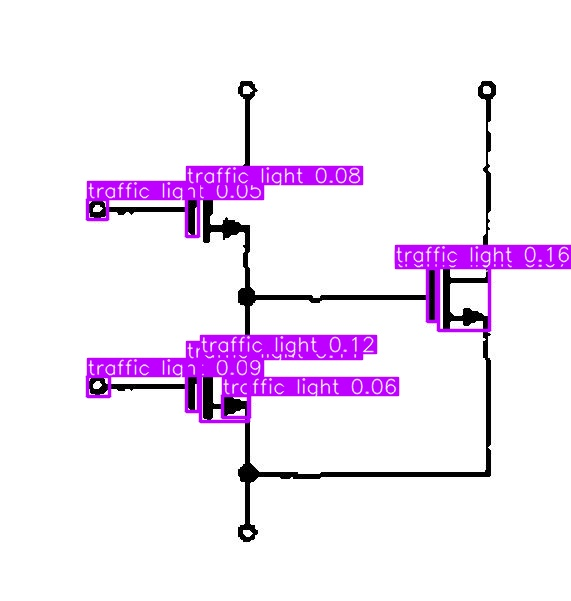
\includegraphics[width=0.4\linewidth]{figures/output_yolo.jpg}
    \caption{\textbf{Output of Yolo11 on a circuit figure.}\\
    As can be seen, the model can only find the prominent patch of the circuit,
    but fails to detect the components precisely in the circuit.}
    \label{fig:yolo_output}
\end{figure}

\subsection{Circuit diagrams in literature work}

Circuit representations in academic literature exhibit significant stylistic variation between papers, as shown in \cref{fig:literature_work}. 
This lack of standardization continues to challenge automated processing approaches.

\begin{figure}[htbp]
    \centering
    \begin{subfigure}[b]{0.3\textwidth}
        \centering
        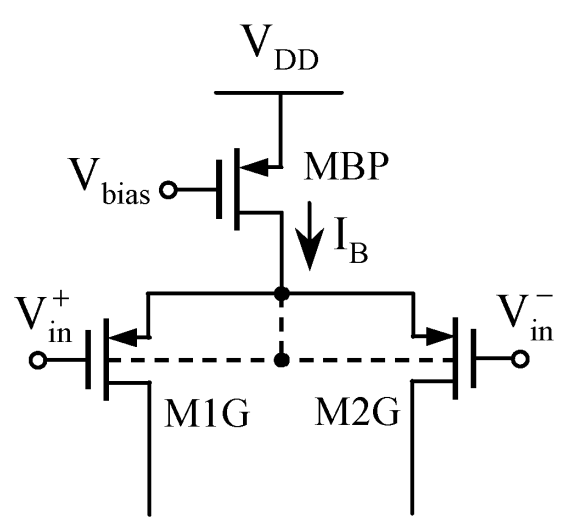
\includegraphics[width=\linewidth]{figures/literature_work1.png}
        \caption{}
        \label{subfig1:literature_work1}
    \end{subfigure}
    \begin{subfigure}[b]{0.5\textwidth}
        \centering
        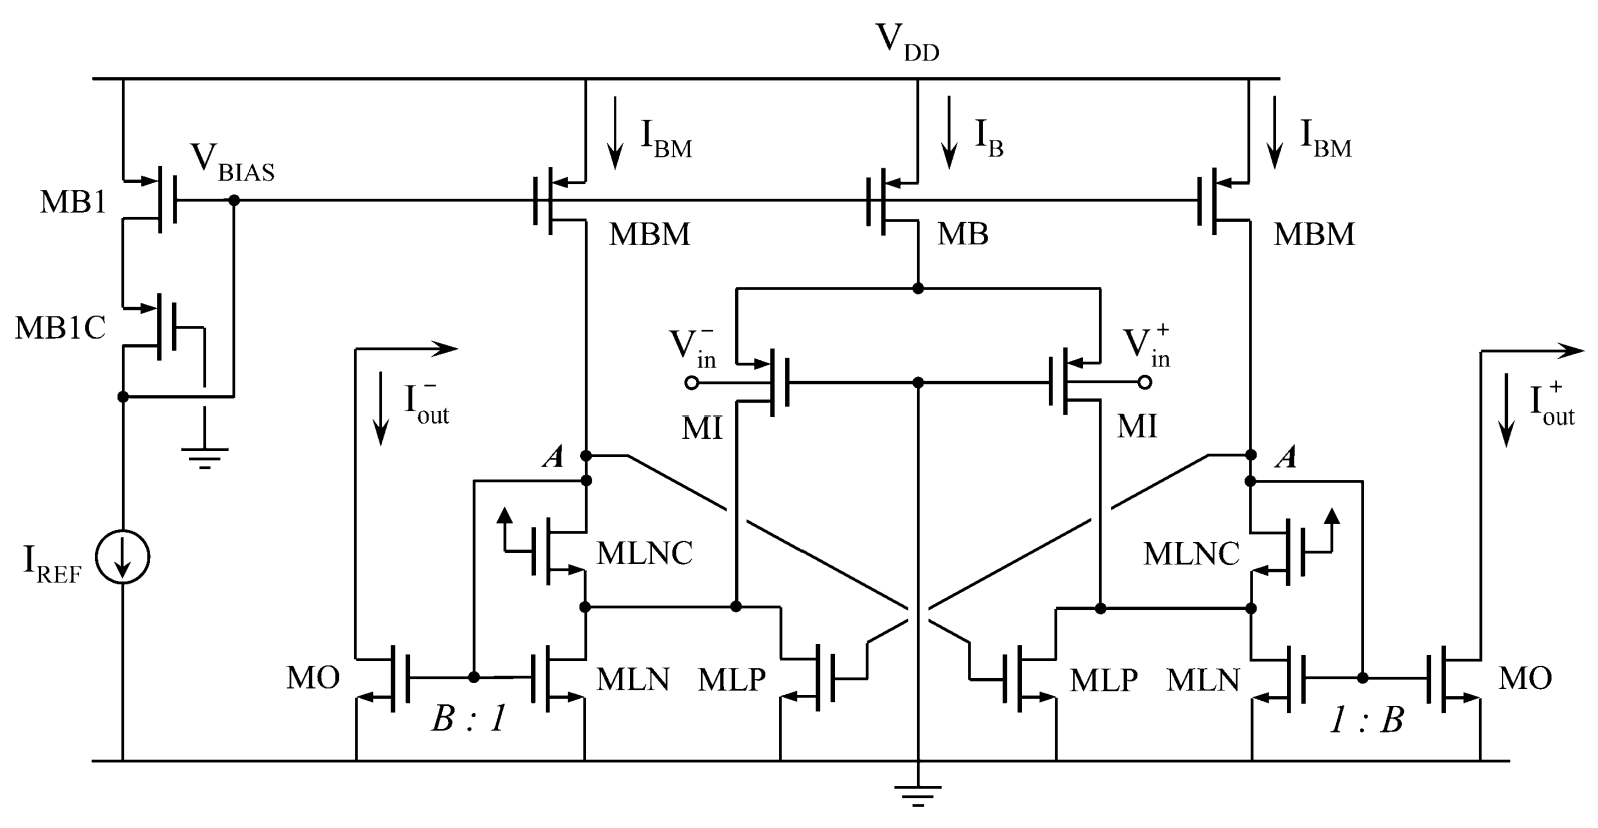
\includegraphics[width=\linewidth]{figures/literature_work2.png}
        \caption{}
        \label{subfig2:literature_work2}
    \end{subfigure}
    \begin{subfigure}[b]{0.45\textwidth}
        \centering
        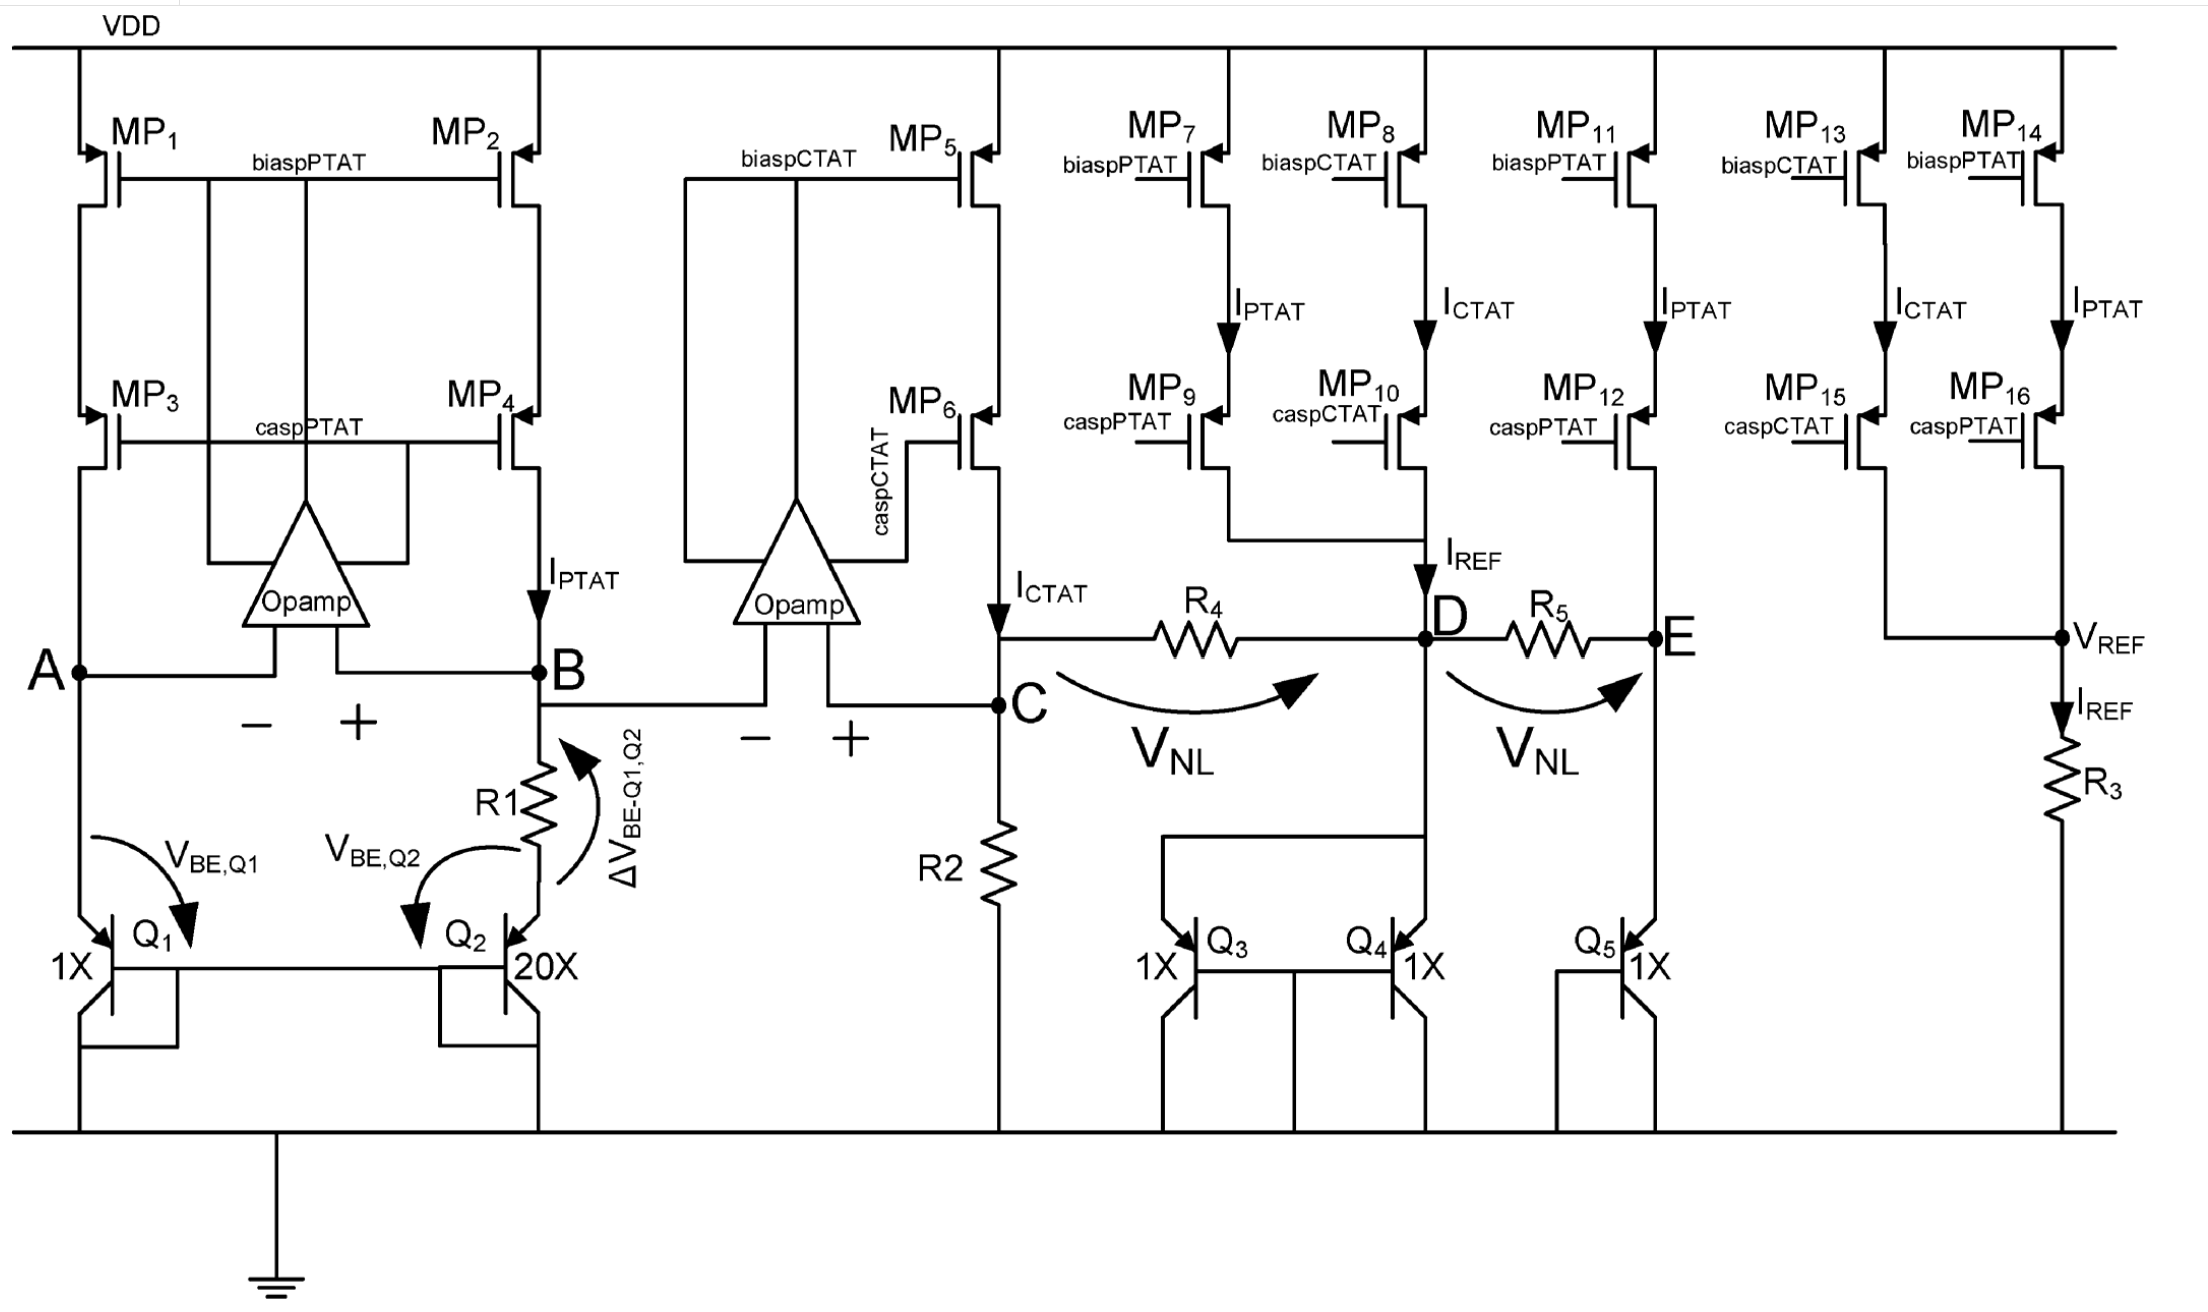
\includegraphics[width=\linewidth]{figures/literature_work3.png}
        \caption{}
        \label{subfig3:literature_work3}
    \end{subfigure}
    \begin{subfigure}[b]{0.45\textwidth}
        \centering
        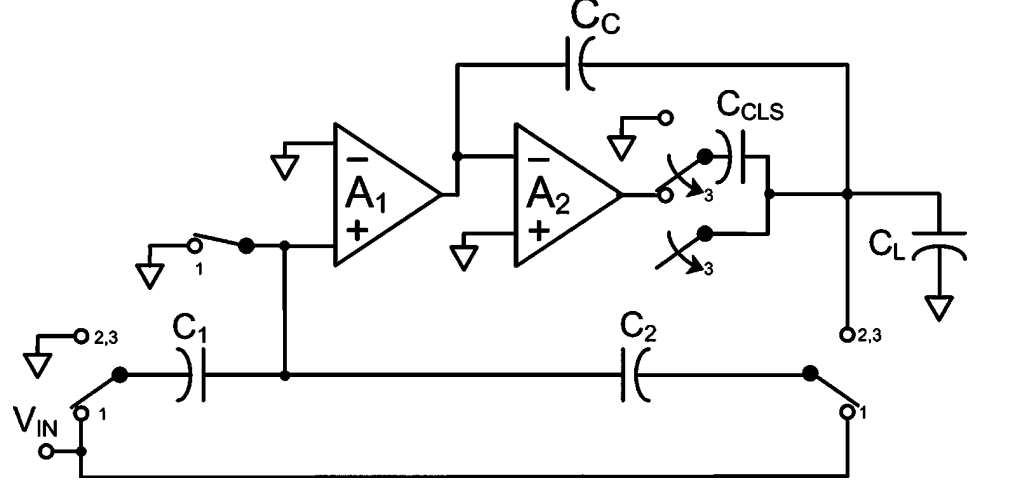
\includegraphics[width=\linewidth]{figures/literature_work4.png}
        \caption{}
        \label{subfig4:literature_work4}
    \end{subfigure}
    \caption{\textbf{Examples of circuit diagrams in literature work.}\\
    As can be seen, diagrams are organized specially for each paper, delivering human logic in a way that is hard to be understood by computers.
    MOSFETs, nodes, junctions, intersections present in different ways.\\
    (a)(b) are from \cite{literature1}, (c) is from \cite{literature2} and (d) is from \cite{literature3}.}
    \label{fig:literature_work}
\end{figure}

\section{Conclusion}\label{sec:conclusion}

In this report, the basic procedures\cite{shi2024amsnet} of generating SPICE netlists from circuit images is reviewed,
followed by some improvements to the algorithm, aiming at applying it to Razavi's textbook\cite{razavi2003}.
Key improvements include: 
\begin{itemize}
\item Adding rescaling steps to template matching
\item Noise-removing algorithm to eliminate unwanted texts, dashed lines and other annotations
\item Finding the balance between thresholds for template matching, sizes of cropped templates, and numbers of templates.
\item Adding OPAMPs to the template library, and making detailed modifications to better handle them.
\end{itemize}
With these improvements, the algorithm is tested on figures from Razavi's book, achieving an average component detection rate of 70\% on 10 randomly selected circuits.
The seemingly low detection rate is largely due to undetected nodes and current arrows, which do not quite affect the netlist generation quality, as discussed in \ref{sec:performance_evaluation}.

To further increase the component detection rate, a PDF version of Razavi's book is used, and comparisons are made between the printed and PDF versions.
It turns out that the PDF version is clearer and smoother, leading to a 14 percentage point increase in component detection rate, from 70\% to 84\%.

However, the algorithm still has limitations, such as confusion between PMOS and NMOS, and incapability of handling some special cases like functional dashed lines, controlled sources and extraordinary junctions.
Moreover, large models without adequate training data connot act well on circuit figures, and the circuit diagrams in literature work are not standardized, making it hard to apply the algorithm to them.

\bibliographystyle{plainnat}
\bibliography{reference}

\appendix

\section{Appendix}

\subsection{Reasons why it's insufficiennt to evade noises through tight boundaries}\label{subsec:tight_boundaries_insufficient}

Current algorithm\cite{shi2024amsnet} evades noises by cropping the templates tightly around the components, thereby not including noises in the boundaries during template matching.
However, during numerous attempts, it has been found that this is not sufficient for the images from Razavi's book, and the reasons are discussed below.

\begin{itemize}
\item The texts,dashed lines and other annotations are sometimes very close to the components: 
This will lead to difficulties in template matching, since the content of the whole window, probably including such noises, is to be compared with the template.
Even if components are successfully detected, the bounding boxes may intersect with such noises, leading to wrong pins being connected because the BFS may start from these intersections instead of true pins.
An example is shown in \cref{subfig1:wrong_pin_example}, where the bounding boxes intersect with the texts and one of three pins of nmos is wrongly handled.
Therefore, it may not work well even with a tight bounding box, which may be affected by the closely placed noises.

Furthermore, the boundaries of OPAMPs almost certainly involve texts like 'A1', 'A2' etc, posing difficulties in template matching. 

\item Sometimes, boundaries simply cannot be chosen too tightly wrapped around the components:
It's observed that the quality of images in Razavi's book is not so good, 
where lines may differ in thickness, and the components are not exactly the same. 
Therefore, a low threshold is needed for template matching. 

With this in mind, it can be concluded that the matching will not be successful sometimes if imposing a tightly wrapped bounding box,
since the roughly sketched components may appear similar locally. 
An example is the template matching of a black node and a NMOS, as shown in \cref{subfig2:wrong_matching_example}, 
where a tight boundary for black node easily crowds out NMOS and results the NMOS undetected.

In other words, the temlate matching has to be implemented in a larger area than the component size, in order to distinguish locally similar components effectively.
However, a larger bounding box risks to include more noises, leading to poor matching results of the component itself. 
\end{itemize} 

\begin{figure}[htbp]
    \centering
    \begin{subfigure}[b]{0.8\textwidth}
        \centering
        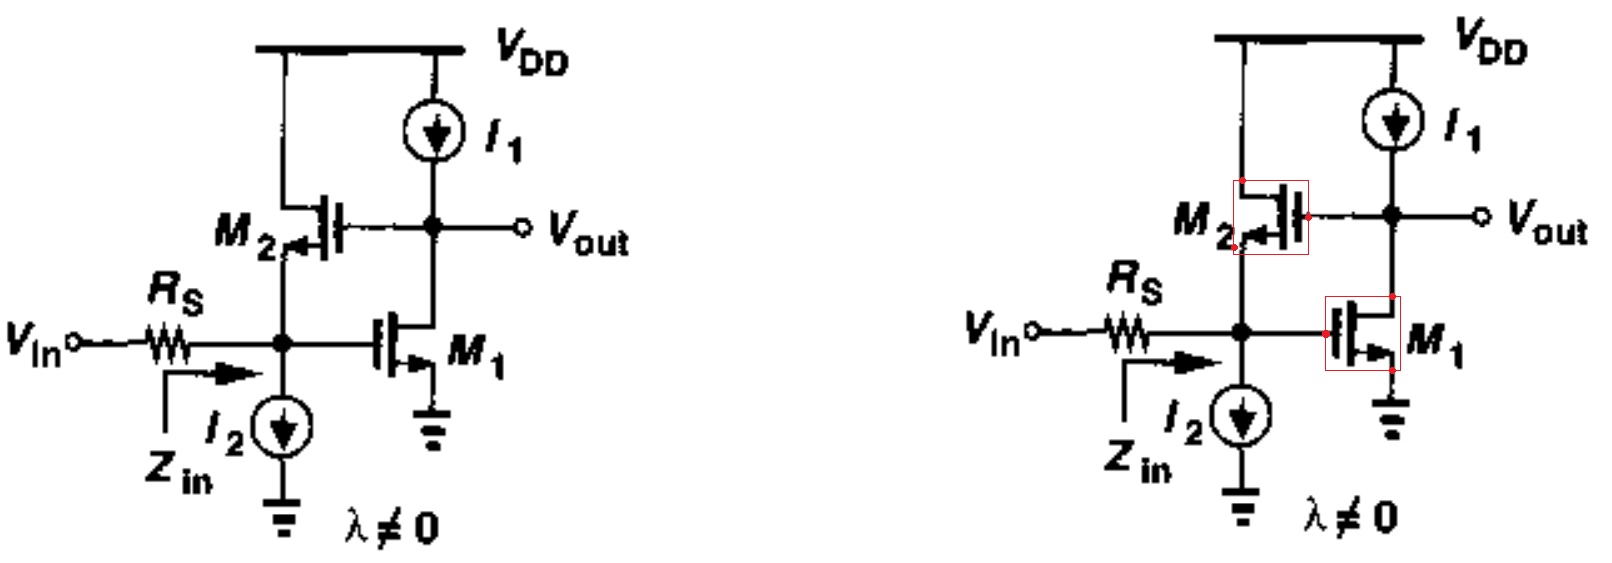
\includegraphics[width=\linewidth]{figures/wrong_pin_example.png}
        \caption{}
        \label{subfig1:wrong_pin_example}
    \end{subfigure}
    \begin{subfigure}[b]{0.5\textwidth}
        \centering
        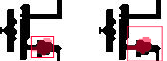
\includegraphics[width=\linewidth]{figures/wrong_matching_example.png}
        \caption{}
        \label{subfig2:wrong_matching_example}
    \end{subfigure}
    \caption{\textbf{Reasons why it's insufficient to evade noises through tight boundaries in Razavi's book.}\\
    \textbf{(a) Texts intersecting with the bounding boxes of components.}
        Boundaries obtained from template matching are presented as rectangular boxes. 
        Starting pixels for BFS are plotted as red dots. One of the three starting points for $M_2$ turns out to be the intersection of the box and texts.
        When searching from pins to connected components, such intersections may replace the right pins, resulting in wrong connections.\\
    \textbf{(b) Demonstrations showing needs for larger boundary boxes during template matching.}
        Take the matching of a black node and an NMOS as an example.
        Due to the poor quality of images, threshold in template matching has to be low enough.
        Such low threshold results that part of NMOS is detected as a black node when matching with a tight box of black node, 
        which is the case in the left figure.
        In the right figure, on the other hand, the bounding box large enough, it's easy to tell the black node from the NMOS in a large window. 
        Therefore, a large bounding box is needed, especially for images with poor quality. But a large boundary will include more noises, leading to poor matching results.}
        \label{fig:insufficient_tight_boundaries}
\end{figure}

\section{Acknowledgements}

I would like to extend my sincere thanks to Zichen Kong and professor Xiyuan Tang for their invaluable suggestions and patient guidance during the development of this report.
Discussions with them have greatly enhanced the quality of this work, and their insights have been instrumental in shaping the final outcome.
I would also like to express my gratitude to Zimo He, Yongqian Peng and professor Yixin Zhu for their support during the whole semester, 
which makes the course more enjoyable and fruitful.

\end{document}